\documentclass[11pt]{article}

\usepackage{amsmath,amsfonts,amssymb,amsthm}
\usepackage{graphicx}
\usepackage{booktabs}
\usepackage{hyperref}
\usepackage{url}
\usepackage{tikz}
\usepackage[margin=1.0in]{geometry}
\usepackage{microtype}
\usepackage{cite}
\usepackage{multirow}
% generated_results.tex
% Auto-generated by src/generate_manifest.py -- DO NOT EDIT DIRECTLY

% Figure 2: Classifier Bootstrap (N=500)
\newcommand{\WidthPearson}{0.5488}
\newcommand{\WidthSpearman}{0.3641}
\newcommand{\WidthMAE}{0.0629}
\newcommand{\UCalPearson}{0.5779}
\newcommand{\UCalSpearman}{0.3650}
\newcommand{\UCalMAE}{0.0429}

% Figure 3: Idealised Scaling Laws
\newcommand{\IdealWidthSlope}{-0.6658}
\newcommand{\IdealWidthCILow}{-0.7235}
\newcommand{\IdealWidthCIHigh}{-0.6082}
\newcommand{\IdealSDSlope}{-0.3399}
\newcommand{\IdealSDCILow}{-0.3865}
\newcommand{\IdealSDCIHigh}{-0.2932}
\newcommand{\IdealUCalSlope}{-0.3344}
\newcommand{\IdealUCalCILow}{-0.3541}
\newcommand{\IdealUCalCIHigh}{-0.3148}

% Figure 5: Non-Monotonic Regimes
\newcommand{\NonMonoRegimeASlope}{-0.685}
\newcommand{\NonMonoRegimeBSlope}{-0.999}
\newcommand{\NonMonoRegimeCSlope}{-1.110}
\newcommand{\NonMonoRegimeDSlope}{-0.794}

% Table 3: CIFAR-10H Crowd Correlations
\newcommand{\CifarBootPearson}{0.5000}
\newcommand{\CifarBootSpearman}{0.5279}
\newcommand{\CifarDisPearson}{0.0007}
\newcommand{\CifarDisSpearman}{0.0007}
\newcommand{\CifarEntPearson}{0.0013}
\newcommand{\CifarEntSpearman}{0.0007}

% Figure 6 & Table 4: Real Tabular Data - Adult
\newcommand{\AdultWidthStart}{0.0061}
\newcommand{\AdultWidthEnd}{0.0293}
\newcommand{\AdultSigmaCalStart}{0.0269}
\newcommand{\AdultSigmaCalEnd}{0.0432}
\newcommand{\AdultEModel}{0.0672}
\newcommand{\AdultDeltaRsq}{0.0494}
\newcommand{\AdultDeltaRsqCILow}{0.0305}
\newcommand{\AdultDeltaRsqCIHigh}{0.0741}

% Figure 6 & Table 4: Real Tabular Data - Bank
\newcommand{\BankWidthStart}{0.0057}
\newcommand{\BankWidthEnd}{0.0375}
\newcommand{\BankSigmaCalStart}{0.0287}
\newcommand{\BankSigmaCalEnd}{0.0556}
\newcommand{\BankEModel}{0.0846}
\newcommand{\BankDeltaRsq}{0.0222}
\newcommand{\BankDeltaRsqCILow}{0.0094}
\newcommand{\BankDeltaRsqCIHigh}{0.0410}

% Figure 6 & Table 4: Real Tabular Data - Spambase
\newcommand{\SpambaseWidthStart}{0.0200}
\newcommand{\SpambaseWidthEnd}{0.1947}
\newcommand{\SpambaseSigmaCalStart}{0.0682}
\newcommand{\SpambaseSigmaCalEnd}{0.0978}
\newcommand{\SpambaseEModel}{0.1338}
\newcommand{\SpambaseDeltaRsq}{0.0011}
\newcommand{\SpambaseDeltaRsqCILow}{0.0000}
\newcommand{\SpambaseDeltaRsqCIHigh}{0.0037}

% Figure 7: Reverse Intervention Refits
\newcommand{\AdultRevEModelStart}{0.0342}
\newcommand{\AdultRevEModelEnd}{0.0986}
\newcommand{\AdultRevWidthStart}{0.0078}
\newcommand{\AdultRevWidthEnd}{0.0070}

\newcommand{\BankRevEModelStart}{0.0436}
\newcommand{\BankRevEModelEnd}{0.1106}
\newcommand{\BankRevWidthStart}{0.0090}
\newcommand{\BankRevWidthEnd}{0.0100}

\newcommand{\SpambaseRevEModelStart}{0.0000}
\newcommand{\SpambaseRevEModelEnd}{0.2003}
\newcommand{\SpambaseRevWidthStart}{0.0200}
\newcommand{\SpambaseRevWidthEnd}{0.0445}


\hypersetup{colorlinks=true,linkcolor=blue,citecolor=blue,urlcolor=blue}

\title{\textbf{The Meaning and Scaling of Venn--Abers Probability Intervals}}

\author{\textbf{Ivan Petej} \\
	\small Department of Computer Science \\
	\small Royal Holloway, University of London \\
	\small \texttt{i.petej@rhul.ac.uk}
}

\date{}

\newtheorem{proposition}{Proposition}
\newtheorem{theorem}{Theorem}
\newtheorem{lemma}{Lemma}

\begin{document}

	\maketitle
	
	\begin{abstract}
		Venn--Abers predictors return two probability values with Venn validity guarantees, $p_0$ and $p_1$, but the interpretation of the interval width $w=p_1-p_0$ has remained unclear. In this paper we study the width through the local block structure of isotonic regression. We show that it is closely related to the inverse effective size of the local PAV block and derive scaling relationships with calibration sample size, score density, label variability, and the slope of the underlying probability curve. The results suggest that Venn--Abers width is primarily a measure of local calibration support rather than a general measure of predictive uncertainty. Controlled scaling experiments recover the predicted behaviour, while bootstrap and crowd-annotation experiments show a much stronger relationship with calibration instability than with label ambiguity. Real-data experiments on three public tabular benchmarks (UCI Adult, UCI Bank Marketing, and UCI Spambase) support this interpretation: deliberately thinning local calibration support monotonically inflates Venn--Abers width and calibration instability while base-model uncertainty is held fixed. In quantitative uncertainty decompositions, Venn--Abers width provides an additional statistically detectable contribution to explaining calibration instability beyond outcome ambiguity and base-model uncertainty ($\Delta R^2 > 0$). These results support the interpretation that Venn--Abers width primarily reflects local calibration support, representing a calibration-specific component of epistemic uncertainty associated with finite local calibration data.
	\end{abstract}

	% ============================================================
\section{Introduction}
	\label{sec:intro}

	Venn--Abers predictors (VAPs) \cite{vovk2014, vovk2015} are probabilistic calibration methods based on the Venn prediction framework. For binary classification they map a scalar scoring rule $s = g(x)$ to a pair of probability values with Venn validity guarantees,
	\begin{equation}
		p_0(s),\qquad p_1(s),
		\label{eq:p0_p1}
	\end{equation}
	obtained by fitting isotonic regression after hypothetically augmenting a calibration sample of size $n$ with the test instance under labels $y=0$ and $y=1$, respectively. For empirical analyses requiring a single scalar summary, we use the midpoint
	\begin{equation}
		\hat p(s)=\frac{p_0(s)+p_1(s)}{2},
		\label{eq:phat_def}
	\end{equation}
	The Venn validity guarantee attaches to the multiprobability pair $(p_0,p_1)$ rather than to this arithmetic midpoint; the standard log-loss merge $p_{\mathrm{VA}}=p_1/(1-p_0+p_1)$ is a distinct point predictor \cite{vovk2015}. The Venn--Abers interval width is
	\begin{equation}
		w_n(s)=p_1(s)-p_0(s).
		\label{eq:wn_def}
	\end{equation}
	We denote the score-conditional Bernoulli outcome variance by
	\begin{equation}
		v(s)=\theta(s)(1-\theta(s)).
		\label{eq:vs_def}
	\end{equation}
	This provides an operational measure of outcome ambiguity at a given score, but need not coincide with irreducible aleatoric uncertainty conditional on the full feature vector $x$. We retain the subscript $n$ when discussing asymptotic dependence on calibration sample size and suppress it in fixed-sample empirical sections.

	While the interval width $w=p_1-p_0$ is frequently used in practice as a confidence score or rejection threshold (e.g., in adversarial example detection \cite{peck2019} and predictive maintenance \cite{johansson2023}), a fundamental question remains: what does the interval width actually measure?

	In this paper we show that contrary to the common intuition that interval width reflects outcome ambiguity ($v(s)$, related to what is commonly termed aleatoric uncertainty), Venn--Abers width is primarily a measure of finite-sample calibration support and local calibration leverage. Using the Greatest Convex Minorant (GCM) representation of isotonic regression, we show that the width is determined by the characteristic active block size $N_{\mathrm{eff}}(s)$ fitted by the Pool Adjacent Violators (PAV) algorithm:
	\begin{equation}
		w_n(s) \approx \frac{1}{N_{\mathrm{eff}}(s)}.
		\label{eq:width_approx_block}
	\end{equation}
	If a test point falls into a large local block with dense calibration support, changing its hypothetical label has minimal leverage on the fitted slope. Conversely, when local calibration data is sparse, active blocks are small, giving the test instance high leverage and producing wide intervals.

	Under a local bias--noise balance for calibration sample size $n$, local score density $f(s)$, true class probability $\theta(s)$, and $\theta'(s)>0$, the usual local isotonic argument gives
	\begin{equation}
		w_n(s) \propto n^{-2/3} f(s)^{-2/3}[v(s)]^{-1/3}[\theta'(s)]^{2/3}.
		\label{eq:intro_scaling}
	\end{equation}
	The negative exponent on the Bernoulli variance $v(s)$ in this expression is a conditional effect: holding score density and slope fixed, higher label noise requires greater local pooling across adjacent observations, enlarging the effective block size and shrinking the width.

	The block-size argument also separates interval width from the sampling variation of the calibrated probability. Treating the local fitted probability as a block mean gives variance of order $v(s)/N_{\mathrm{eff}}(s)$. For this reason we also define
	\begin{equation}
		U_{{\rm cal},n}(s) = \sqrt{\hat p(s)(1-\hat p(s))\,w_n(s)},
		\label{eq:intro_ucal}
	\end{equation}
	which has the predicted isotonic $n^{-1/3}$ scale. We use this quantity as an index of calibration instability rather than as an exact standard error. We refer primarily to the interval width $w_n$ as local calibration leverage, or equivalently inverse effective calibration support. In the usual aleatoric--epistemic terminology, the uncertainty represented by the width can be viewed as a calibration-specific component of epistemic uncertainty arising from finite local calibration information.

	We test these relationships in a number of experiments. These include monotonic and non-monotonic synthetic examples, bootstrap resampling, a crowd-annotation simulation, and controlled local support interventions on three real-world tabular benchmarks (UCI Adult, UCI Bank Marketing, and UCI Spambase). We also increase the calibration sample size to check whether the finite-sample density, ambiguity, and slope coefficients move towards the values suggested by the scaling argument. The results are broadly consistent with the proposed interpretation. In the real-data experiments, thinning local calibration support increases Venn--Abers width and pointwise calibration instability while base-model epistemic uncertainty is held fixed by construction. In quantitative decompositions across held-out test points, outcome ambiguity explains baseline Bernoulli variability, while Venn--Abers width provides an additional statistically detectable contribution across all three datasets ($\Delta R^2 = +\AdultDeltaRsq{}$ on Adult, $+\BankDeltaRsq{}$ on Bank, and $+\SpambaseDeltaRsq{}$ on Spambase; all 95\% bootstrap CIs exclude zero), consistent with width capturing calibration-support information distinct from outcome ambiguity and base-model bootstrap variability.

	% ============================================================
\section{Related Work}
	\label{sec:related}

	\paragraph{Venn--Abers and Conformal Calibration.}
	Venn--Abers predictors were introduced by Vovk and Petej \cite{vovk2014} as a class of Venn predictors based on isotonic regression. Their main attraction is probabilistic validity under exchangeability. A computationally efficient version was subsequently developed in \cite{vovk2015} using the Pool Adjacent Violators algorithm. Subsequent work has considered multi-class Venn--Abers prediction \cite{manokhin2017multiclass}, extensions to predictive distributions \cite{nouretdinov2018ivapdist}, and more recently Venn--Abers methods for regression \cite{petej2026regressors}. Unlike standard conformal predictors, which usually return prediction sets, Venn--Abers predictors return a pair of probabilities and can also be reduced to a single probability prediction when required.

	\paragraph{Asymptotic Theory of Isotonic Regression.}
	The behaviour of Venn--Abers calibration is closely connected to isotonic regression. The pointwise isotonic estimator has the well-known cube-root rate rather than the usual $n^{-1/2}$ rate, with its limiting behaviour described through the greatest convex minorant of Brownian motion with drift \cite{groeneboom1985}. The characteristic size and behaviour of the local active blocks fitted by isotonic regression have been studied extensively in shape-constrained inference \cite{wright1981, robertson1988, groeneboom2014, han2022}. The aim here is not to reproduce this theory, but to use the local isotonic block structure to understand the additional quantity $p_1-p_0$ produced by Venn--Abers calibration.

	\paragraph{Finite-Sample Calibration and Uncertainty.}
	Calibration of modern classification models has traditionally been evaluated through aggregate summary metrics such as Expected Calibration Error (ECE), though finite-sample estimators can exhibit substantial empirical bias and variance \cite{kumar2019, vaicenavicius2019}. Recent work has focused on distribution-free guarantees, adaptive binning, and finite-sample confidence intervals for calibration mappings \cite{gupta2020}. In modern classification systems, estimating uncalibrated model confidence, calibration errors, and selective abstention has likewise drawn growing attention \cite{kumar2019}. Our work complements these directions by examining what the interval width of a non-parametric calibrator directly reflects.

	\subsection{Interpreting Venn--Abers Intervals}
	Venn--Abers intervals have been used in several different ways. In the original work, the pair $[p_0,p_1]$ is part of the Venn multiprobabilistic construction. In later applications the width $p_1-p_0$ has also been used as a confidence or rejection score, for example in adversarial example detection \cite{peck2019} and predictive maintenance \cite{johansson2023}.

	There has been less work on what the width itself measures. In particular, the same numerical width could in principle be attributed to label ambiguity, lack of local calibration data, or instability of the fitted calibration curve. We separate these effects experimentally and study how the width changes with local density, Bernoulli variance, and slope.

	% ============================================================
\section{Problem Setup and Notation}
	\label{sec:setup}
	
	Let $\mathcal{X}$ denote the input space and $\mathcal{Y} = \{0, 1\}$ denote the binary label space. We assume access to a training dataset and a calibration dataset $\mathcal{D}_{\text{cal}} = \{(x_i, y_i)\}_{i=1}^n$. 
	
	A base machine learning model is trained on proper training data to produce a score function $g: \mathcal{X} \to \mathbb{R}$. For a given calibration sample $(x_i, y_i)$, we compute the calibration score $s_i = g(x_i)$. The scores are sorted such that $s_1 \le s_2 \le \dots \le s_n$, with $y_1, \dots, y_n$ representing the corresponding binary labels. We model the label generating distribution as $y_i \mid s_i \sim \text{Bernoulli}(\theta(s_i))$, where $\theta(s)$ is the true latent probability curve mapping scores to class probabilities. We write $f(s)$ for the probability density of the calibration scores. Thus, in a score interval of width $\Delta s$ around an interior point $s$, the expected number of calibration observations is approximately $n f(s)\Delta s$.
	
	% ============================================================
	\section{Venn--Abers Predictors}
	\label{sec:venn_abers}
	
	Venn--Abers predictors calibrate the output of a base scoring model $g: \mathcal{X} \to \mathbb{R}$ using the sorted calibration scores $s_1 \le s_2 \le \dots \le s_n$. Given a test input $x$ with score $s = g(x)$, we consider two hypothetical scenarios:
	\begin{enumerate}
		\item If the true label of $x$ were $0$, we insert the pair $(s, 0)$ into the calibration sequence, sort the augmented sequence, and fit a monotonic mapping using the Pool Adjacent Violators (PAV) algorithm. Let $p_0(s)$ be the calibrated probability assigned to $s$ under this mapping.
		\item If the true label of $x$ were $1$, we insert the pair $(s, 1)$ into the calibration sequence, sort, and fit PAV. Let $p_1(s)$ be the calibrated probability assigned to $s$ under this mapping.
	\end{enumerate}
	
	The Venn--Abers predictor outputs the interval $[p_0(s), p_1(s)]$. By construction, $p_0(s) < p_1(s)$ strictly: hypothesizing label $1$ can only raise the fitted value at $s$ relative to hypothesizing label $0$, and the two PAV fits assign it to overlapping but distinct level sets. As introduced in Section~\ref{sec:intro}, for empirical analyses we summarize the pair by the midpoint $\hat{p}(s)$, while the interval width is $w_n(s)$:
	\begin{equation}
		\hat{p}(s) = \frac{p_0(s) + p_1(s)}{2}, \quad w_n(s) = p_1(s) - p_0(s).
	\end{equation}
	The pair $(p_0(s), p_1(s))$ is part of the multiprobabilistic validity construction of Venn--Abers predictors \cite{vovk2015}. It should not be interpreted as a classical confidence interval for an unknown Bernoulli probability. The experiments use the open-source \texttt{venn-abers} Python package \cite{vennaberspkg} directly, or an accelerated implementation that is tested for numerical equivalence to the package on continuous, tied, and bootstrap-resampled scores.
	
	% ============================================================
	\section{Theory: Asymptotic Scaling Laws of Venn--Abers Intervals}
	\label{sec:theory}
	
	In this section we derive a local approximation for the Venn--Abers interval width using the block structure of isotonic regression. The derivation is heuristic, but it gives quantities which can be checked directly in the experiments.
	
	\subsection{GCM Representation of Isotonic Regression}
	
	Let $(s_1, y_1), \dots, (s_n, y_n)$ be the sorted calibration points. We define the cumulative sum diagram as the set of points $P_k = (k, S_k)$ for $k = 0, \dots, n$, where $S_0 = 0$ and $S_k = \sum_{i=1}^k y_i$. 
	
	Isotonic regression of $y$ on $s$ corresponds to finding the Greatest Convex Minorant (GCM) of this diagram. The fitted value $\hat{y}_i$ is the slope of the GCM at index $i$. The GCM consists of linear segments (active blocks) over which the fitted probabilities are constant.
	
	When we insert a test point $s$ with label $y \in \{0, 1\}$, we insert a node in the diagram at the appropriate sorted index $j$.
	\begin{itemize}
		\item Inserting $y = 0$ leaves the cumulative sum unchanged for subsequent points but shifts their index by $1$: later CSD points move purely horizontally.
		\item Inserting $y = 1$ shifts both the index and the cumulative sum of subsequent points by $1$: later CSD points move diagonally, not just upward.
	\end{itemize}
	This conceptual relationship is illustrated in Figure~\ref{fig:gcm_illustration}.
	
	\begin{figure}[ht]
		\centering
		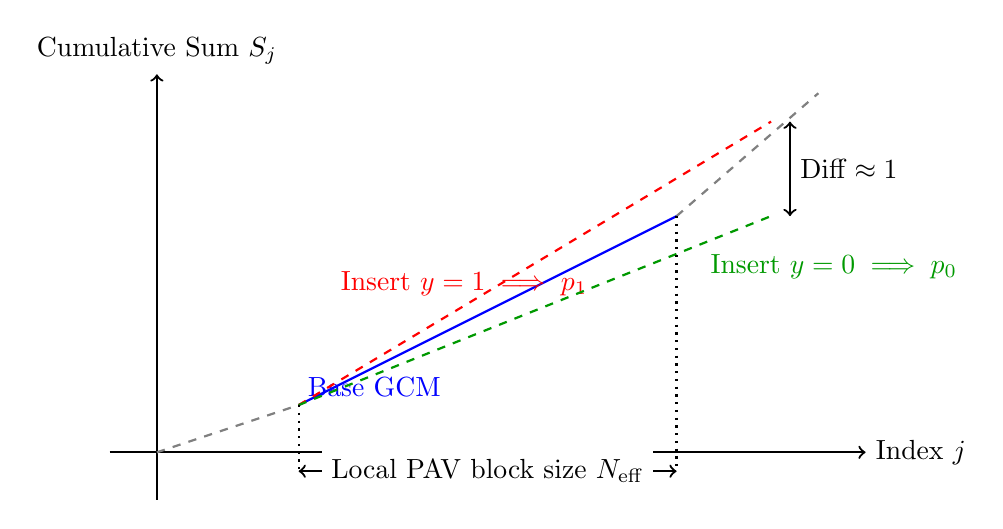
\begin{tikzpicture}[scale=1.2]
			% Axes
			\draw[->, thick] (-0.5, 0) -- (7.5, 0) node[right] {Index $j$};
			\draw[->, thick] (0, -0.5) -- (0, 4) node[above] {Cumulative Sum $S_j$};
			
			% Original GCM pieces
			\draw[gray, dashed, thick] (0,0) -- (1.5, 0.5);
			\draw[gray, dashed, thick] (5.5, 2.5) -- (7, 3.8);
			
			% Active Block (N=4), pre-insertion
			\draw[blue, thick] (1.5, 0.5) -- (5.5, 2.5) node[pos=0.2, below] {Base GCM};

			% Adding y=1: subsequent index AND cumulative sum both shift by 1 (diagonal move)
			\draw[red, thick, dashed] (1.5, 0.5) -- (6.5, 3.5) node[pos=0.35, above] {Insert $y=1 \implies p_1$};

			% Adding y=0: subsequent index shifts by 1, cumulative sum unchanged (horizontal move)
			\draw[green!60!black, thick, dashed] (1.5, 0.5) -- (6.5, 2.5) node[pos=0.85, below right] {Insert $y=0 \implies p_0$};

			% Interval Width Bracket (both new endpoints share the same shifted index 6.5)
			\draw[<->, thick] (6.7, 2.5) -- (6.7, 3.5) node[midway, right] {Diff $\approx 1$};

			% N bracket (pre-insertion block size)
			\draw[<->, thick] (1.5, -0.2) -- (5.5, -0.2) node[midway, fill=white] {Local PAV block size $N_{\mathrm{eff}}$};
			\draw[dotted, thick] (1.5, 0.5) -- (1.5, -0.2);
			\draw[dotted, thick] (5.5, 2.5) -- (5.5, -0.2);
		\end{tikzpicture}
		\caption{Conceptual illustration of the GCM logic. The test point falls into a local active block of length $N$. Inserting the test point shifts the index of every subsequent CSD point by $1$; with hypothesized label $y=1$ this also shifts their cumulative sum up by $1$ (a diagonal move), while $y=0$ leaves the cumulative sum unchanged (a horizontal move). The resulting difference in the GCM slope out to the shifted endpoint gives the probability interval width $p_1 - p_0$, approximately $1/N$.}
		\label{fig:gcm_illustration}
	\end{figure}
	
	Suppose the test point $s$ falls within an active block of length $N$ in the base GCM. Let the sum of labels in this block be $K$, so the baseline slope (probability) is $K/N$.
	\begin{itemize}
		\item Inserting $(s, 0)$ into the block yields a fitted probability $p_0 \approx \frac{K}{N+1}$.
		\item Inserting $(s, 1)$ into the block yields a fitted probability $p_1 \approx \frac{K+1}{N+1}$.
	\end{itemize}
	Assuming the insertion of a single point does not trigger cascading merges of adjacent blocks, the interval width is:
	\begin{equation}
		w(s) = p_1 - p_0 \approx \frac{K+1}{N+1} - \frac{K}{N+1} = \frac{1}{N+1} \approx \frac{1}{N}.
		\label{eq:width_block}
	\end{equation}
	Equation~\ref{eq:width_block} shows that the Venn--Abers interval width is inversely proportional to the local block size $N$ of the isotonic regression.
	
	\subsection{Derivation of Local Block Size}
	
	To determine how the active block size behaves, we use the usual local bias--noise balance underlying cube-root isotonic asymptotics. Let the calibration sample size be $n$, let $f(s)$ denote the local probability density of scores, and let
	\begin{equation}
		v(s)=\theta(s)(1-\theta(s)).
	\end{equation}
	Consider a local score interval of width $\Delta s$ around an interior score $s$. Its expected number of calibration observations is
	\begin{equation}
		N \approx n f(s)\Delta s.
		\label{eq:block_count_n}
	\end{equation}
	
	\paragraph{1. Systematic Variation.}
	When $\theta'(s)>0$, the change in the true probability across the interval is of order
	\begin{equation}
		\theta'(s)\Delta s.
	\end{equation}
	
	\paragraph{2. Statistical Noise.}
	The empirical mean of a block containing $N$ Bernoulli observations has standard deviation of order
	\begin{equation}
		\sqrt{\frac{v(s)}{N}}
		\approx
		\sqrt{\frac{v(s)}{n f(s)\Delta s}}.
	\end{equation}
	
	\paragraph{3. Local Balance.}
	Balancing the systematic change against the local noise gives
	\begin{equation}
		\theta'(s)\Delta s
		\approx
		\sqrt{\frac{v(s)}{n f(s)\Delta s}},
	\end{equation}
	and therefore
	\begin{equation}
		(\Delta s)^3
		\approx
		\frac{v(s)}{n f(s)[\theta'(s)]^2}.
		\label{eq:delta_regular}
	\end{equation}
	Substituting Equation~\ref{eq:delta_regular} into Equation~\ref{eq:block_count_n} gives the characteristic active-block size
	\begin{equation}
		N_{\mathrm{eff}}(s)
		\propto
		n^{2/3}f(s)^{2/3}v(s)^{1/3}[\theta'(s)]^{-2/3}.
		\label{eq:block_scaling}
	\end{equation}
	Using $w(s)\approx 1/N_{\mathrm{eff}}(s)$ then gives the following scaling relationship.
	
	\begin{proposition}[Heuristic Local Scaling Law]
		Assume that $s$ is an interior point, $f(s)>0$, $0<\theta(s)<1$, and that $f$ and $\theta$ are locally smooth with $\theta'(s)>0$. Assume further that the local PAV block is in the regular isotonic regime and that its characteristic scale is determined by the bias--noise balance above. Then
		\begin{equation}
			w_n(s)
			\propto
			n^{-2/3}f(s)^{-2/3}
			[\theta(s)(1-\theta(s))]^{-1/3}
			[\theta'(s)]^{2/3},
			\label{eq:scaling_law_final}
		\end{equation}
		up to multiplicative constants and finite-sample active-block effects.
	\end{proposition}
	
	The proposition is intended as an asymptotic scaling relationship rather than a formal limit theorem. Its $n^{-2/3}$ block-influence rate is also consistent with the standard $n^{-1/3}$ pointwise rate of isotonic regression: the interval width behaves like inverse local block size, whereas the fitted block mean fluctuates on the square-root scale of that inverse block size.

	Equation~\ref{eq:scaling_law_final} can also be reached as a corollary of the same balance stated once in the score scale where the calibration curve is the identity, where the $\theta'(s)$ factor is absent by construction; Appendix~\ref{sec:appendix_invariance} gives this route and uses it to show that Equation~\ref{eq:scaling_law_final} is automatically invariant under strictly increasing score transformations.
	
	\subsection{From Interval Width to Probability-Scale Calibration Instability}
	\label{subsec:ucal_theory}
	
	The block-size interpretation suggests that interval width and calibration variability should not be expected to have the same rate. Within a local block, the fitted probability is approximately a Bernoulli block mean, so
	\begin{equation}
		\operatorname{Var}\{\hat p(s)\}
		\asymp
		\frac{v(s)}{N_{\mathrm{eff}}(s)}.
	\end{equation}
	Using $w_n(s)\asymp1/N_{\mathrm{eff}}(s)$ gives
	\begin{equation}
		\operatorname{Var}\{\hat p(s)\}
		\asymp
		v(s)w_n(s),
		\label{eq:variance_width_relation}
	\end{equation}
	and therefore the characteristic probability-scale fluctuation is
	\begin{equation}
		U_{{\rm cal},n}(s)
		=
		\sqrt{\hat p(s)(1-\hat p(s))\,w_n(s)}.
		\label{eq:ucal}
	\end{equation}
	Combining Equation~\ref{eq:ucal} with Proposition~1 predicts
	\begin{equation}
		U_{{\rm cal},n}(s)
		\propto
		n^{-1/3}f(s)^{-1/3}
		[v(s)]^{1/3}
		[\theta'(s)]^{1/3},
		\label{eq:ucal_scaling}
	\end{equation}
	up to constants and local active-block effects. Thus, width has the inverse-block or leverage rate $n^{-2/3}$, whereas the probability-scale calibration instability has the usual cube-root rate $n^{-1/3}$. In fixed-sample empirical sections, where calibration sample size $n$ is held constant, we suppress the subscript $n$ and write $w(s)$ and $U_{\mathrm{cal}}(s)$. We use $U_{\mathrm{cal}}$ as an instability index rather than as an exact standard-error estimator: the proportionality constant can depend on local geometry, and our finite-sample experiments show substantial pointwise variation around this relationship.
	
	\subsection{Interpretation of the Scaling Law}
	
	Equation~\ref{eq:scaling_law_final} separates four local effects:
	\begin{itemize}
		\item \textbf{Calibration size ($n^{-2/3}$):} Increasing the calibration sample increases the characteristic local PAV block size and reduces the interval width. To first order, doubling local calibration support has a larger effect on width than would be suggested by a standard $n^{-1/2}$ sampling rate.
		\item \textbf{Score density ($f^{-2/3}$):} Holding the other local quantities fixed, dense score regions have larger active blocks and narrower intervals. Sparse regions have smaller effective support and larger local calibration leverage.
		\item \textbf{Bernoulli variance ($v^{-1/3}$):} Holding score density and local slope fixed, larger $v(s)=\theta(s)(1-\theta(s))$ increases the amount of pooling required to overcome local noise and therefore reduces the width. This is a \emph{partial} dependence, not a statement that ambiguous observations must have narrow intervals in an arbitrary model. For example, in a logistic family the local slope co-varies with $v(s)$, and substituting $\theta'(s)\propto v(s)$ reverses the net dependence to $w\propto v^{1/3}$.
		\item \textbf{Local slope ($[\theta']^{2/3}$):} A steeper probability curve produces greater systematic variation over a short score interval, limiting the amount of pooling and leading to smaller blocks and wider intervals.
	\end{itemize}
	
	We interpret the width therefore as a local sensitivity or leverage property generated by the calibration procedure, decomposed structurally as:
	\begin{equation}
		w_n(s) \;\sim\; \underbrace{n^{-2/3}f(s)^{-2/3}}_{\text{calibration leverage (inverse support)}} \;\times\; \underbrace{v(s)^{-1/3}}_{\text{outcome variability}} \;\times\; \underbrace{[\theta'(s)]^{2/3}}_{\text{local geometry}}.
		\label{eq:scaling_decomp}
	\end{equation}
	Width is thus not one of the conventional predictive uncertainty components: it is an empirical sensitivity measure arising from the calibration step, influenced by score-conditional outcome noise but fundamentally distinct from it. We refer primarily to the width as local calibration leverage, or equivalently inverse effective calibration support. In the conventional aleatoric--epistemic taxonomy, it can be viewed as a calibration-specific component of epistemic uncertainty arising from finite local calibration data. Equation~\ref{eq:ucal} incorporates the score-conditional outcome variance $v(s)$ back into the expression when the quantity of interest is probability-scale instability.
	
	\subsection{Non-Monotonicity and Alternative Scaling Regimes}
	\label{subsec:non_monotonic_theory}
	
	The regular derivation assumes a non-zero first-order local trend. More generally, suppose the first non-vanishing local change around $s_0$ is of order $\alpha$,
	\begin{equation}
		\theta(s_0+h)-\theta(s_0)
		\asymp
		c\,\operatorname{sign}(h)|h|^{\alpha},
	\end{equation}
	for some $\alpha\ge1$. Balancing $c(\Delta s)^\alpha$ against the Bernoulli sampling noise gives
	\begin{equation}
		w_n(s_0)
		\propto
		[nf(s_0)]^{-\frac{2\alpha}{2\alpha+1}}
		v(s_0)^{-\frac{1}{2\alpha+1}}
		c^{\frac{2}{2\alpha+1}}.
		\label{eq:general_order_scaling}
	\end{equation}
	The regular case $\alpha=1$ gives the $n^{-2/3}$ rate. An order-two flat or kink-like regime gives $n^{-4/5}$, while a smooth monotone cubic flat point with first non-zero derivative of order three gives $n^{-6/7}$. This distinction is useful because a twice-differentiable monotone function cannot have an interior point with $\theta'(s_0)=0$ and $\theta''(s_0)\ne0$ while remaining monotone on both sides. As shown in Appendix~\ref{sec:appendix_invariance}, Equation~\ref{eq:general_order_scaling} is not a separate calculation from Equation~\ref{eq:scaling_law_final}: both follow from the same balance in the canonical score scale, at general $\alpha$ and at $\alpha=1$ respectively.
	
	In a genuine monotonicity-violating region, a different regime applies. Let $\theta^*$ denote the population isotonic projection of $\theta$. If $s_0$ lies inside a flat population block $I=[a,b]$ induced by a persistent monotonicity violation, the empirical PAV block contains approximately
	\begin{equation}
		N_I \approx n\int_a^b f(t)\,dt
	\end{equation}
	observations. The interval width is then of order
	\begin{equation}
		w_n(s_0)
		\asymp
		\frac{1}{n\int_a^b f(t)\,dt}
		=
		O(n^{-1}),
		\label{eq:scaling_law_violation}
	\end{equation}
	provided the limiting pooled region has non-vanishing mass. Thus, the $n^{-1}$ regime is associated with a macroscopic population-level pooling interval rather than with a local derivative alone.
	
	In these examples the width depends on the geometry of the isotonic projection. In a regular increasing region we obtain the usual local cube-root block scale. At a higher-order flat point the rate changes, while a persistent violation can force the PAV algorithm to pool a non-vanishing part of the local score range into one flat block. In the latter case the width can fall at the faster $n^{-1}$ rate, but the fitted calibration curve has also lost local resolution.
	
	% ============================================================
	\section{Experimental Setup}
	\label{sec:experiments}
	
	We use four sets of experiments. The first group consists of controlled one-dimensional simulations used to test the scaling relationships. We then use bootstrap resampling and a crowd-annotation simulation to compare interval width with calibration instability and label ambiguity. Finally, we evaluate real-world tabular classification datasets under controlled local support thinning and training subsampling to test the calibration-support interpretation in a practical machine learning setting.
	
	\subsection{Synthetic Data Generation}
	We distinguish three controlled synthetic experimental protocols to validate different aspects of the asymptotic theory:
	\begin{enumerate}
		\item \textbf{Idealised Sample-Size Scaling (Figure~\ref{fig:idealised_scaling}):} To test the pure sample-size scaling exponents ($-2/3$ for interval width and $-1/3$ for pointwise standard deviation and $U_{\mathrm{cal}}$), we generate scores $S \sim U[0,1]$ with $Y\mid S=s\sim\operatorname{Bernoulli}(0.2+0.6s)$. We evaluate a fixed interior score $s_0=0.5$ at calibration sizes $n\in\{500,1000,2000,4000,8000,16000,32000\}$ using $R=200$ independent Monte Carlo repetitions per sample size.
		\item \textbf{Multivariate Asymptotic Scaling ($W_2$ Factorial Design, Table~\ref{tab:exponent_convergence} and Equation~\ref{eq:pooled_w2}):} To verify the joint dependence on score density $f(s)$, Bernoulli variance $v(s)=\theta(s)(1-\theta(s))$, and curve derivative $\theta'(s)$ in Equation~\ref{eq:scaling_law_final}, we use four score-density families (uniform, centered truncated Gaussian, shifted truncated Gaussian, and asymmetric Beta), six monotone probability curves (four sigmoidal variants and two power curves), and 14 interior evaluation scores $s\in[-0.65,0.65]$. We evaluate calibration sizes $n\in\{500,1000,2000,4000,8000,16000,32000\}$, with the number of Monte Carlo repetitions decreasing from eight at the smaller sizes to two at $n=32000$.
		\item \textbf{Non-Monotonic Geometric Regimes (Figure~\ref{fig:non_monotonic_scaling_laws}):} To evaluate the effect of monotonicity violations and higher-order local geometry, we use scores $S\sim U[-1,1]$ under four regimes: regular monotonic, globally decreasing, a middle-peak monotonicity violation, and an order-two monotone flat/kink regime. We use calibration sizes $n\in\{100,200,400,800,1600,3200\}$ with $R=500$ Monte Carlo repetitions per size.
	\end{enumerate}
	

	\subsection{Real-World Binary Tabular Datasets}
	\label{subsec:real_data_setup}

	To evaluate the calibration-support interpretation on realistic machine learning tasks, we conduct experiments on three widely studied public binary classification benchmarks:
	\begin{itemize}
		\item \textbf{UCI Adult ($N=48{,}842$):} Census income prediction (binary target: income $>$\$50{,}000/year).
		\item \textbf{UCI Bank Marketing ($N=45{,}211$):} Direct marketing campaign response (binary target: term deposit subscription).
		\item \textbf{UCI Spambase ($N=4{,}601$):} Email classification into spam versus non-spam based on word and character frequencies, representing a smaller-sample regime.
	\end{itemize}
	Each dataset is partitioned using a reproducible stratified split into 50\% training, 25\% calibration, and 25\% held-out test data. Categorical features are encoded using standard ordinal preprocessing. As the base classification learner, we train a gradient-boosted decision tree ensemble (\texttt{HistGradientBoostingClassifier}, maximum tree depth 4, learning rate 0.05, 200 boosting iterations). On the held-out test set, the base classifiers achieve classification accuracy of 87.6\% on Adult, 91.0\% on Bank Marketing, and 94.8\% on Spambase.

	\paragraph{Quantifying Three Sources of Uncertainty.}
	Following the conceptual framework of Section~\ref{sec:theory}, we distinguish three operational uncertainty quantities on the held-out test points:
	\begin{enumerate}
		\item \textbf{Outcome Ambiguity Proxy ($A(x)$):} The estimated conditional label variability, defined as $A(x) = \hat p(x)(1 - \hat p(x))$, where $\hat p(x) = (p_0(x) + p_1(x))/2$ is the Venn--Abers calibrated probability midpoint. We state explicitly that on real observational datasets this represents an estimated proxy for outcome ambiguity rather than directly observed irreducible Bayes error.
		\item \textbf{Base-Model Epistemic Uncertainty ($E_{\mathrm{model}}(x)$):} Epistemic uncertainty in the base predictor due to finite training sample size. We estimate $E_{\mathrm{model}}(x) = \mathrm{SD}_b(g_b(x))$ by repeatedly refitting the base classifier across $B_{\mathrm{model}} = 100$ bootstrap resamples of the training partition while keeping the calibration set fixed.
		\item \textbf{Calibration Epistemic Uncertainty / Support ($w(x)$):} The Venn--Abers interval width $w(x) = p_1(x) - p_0(x)$ and corresponding instability index $U_{\mathrm{cal}}(x) = \sqrt{A(x) w(x)}$, capturing finite local support for the fitted calibration mapping.
	\end{enumerate}

	\paragraph{Intervention on Local Calibration Support.}
	To test the central hypothesis that Venn--Abers width captures local calibration leverage rather than generic predictive or base-model epistemic uncertainty, we deliberately alter local calibration support while keeping the trained base model and test points strictly fixed. 
	For each dataset, we select representative held-out test points spanning score space (targeting scores around $0.20, 0.35, 0.50, 0.65, 0.80$). Around each test point's calibration score $s_0$, we define a local rank-based neighbourhood comprising the nearest 10\% of calibration observations in score rank space.
	We then progressively thin only the calibration observations in that local neighbourhood to retained fractions of $100\%$, $75\%$, $50\%$, $25\%$, and $12.5\%$, leaving all calibration points outside the neighbourhood unchanged. Random thinning is repeated across $R_{\mathrm{thin}} = 100$ replicates. For each thinning fraction, we evaluate the resulting interval width $w$ and estimate pointwise calibration bootstrap instability $\sigma_{\mathrm{cal}}(x) = \mathrm{SD}_b(\hat p_b(x))$ across $B_{\mathrm{cal}} = 100$ bootstrap draws of the thinned calibration set.

	\paragraph{Reverse Intervention on Training Support.}
	To distinguish sensitivity to calibration support from sensitivity to base-model training support, we also conduct a complementary reverse intervention: keeping the calibration and test partitions fixed, we refit the base classifier on progressively smaller training subsets (retained fractions of $100\%$, $75\%$, $50\%$, and $25\%$). We record the response of base-model uncertainty $E_{\mathrm{model}}(x)$ and Venn--Abers width $w(x)$.

	% ============================================================
	\section{Results and Empirical Analysis}
	\label{sec:results}
	
	\subsection{Resampling Analysis and Calibration Instability}
	
	We first compare interval width with the variability obtained by repeatedly drawing a new calibration sample from the same distribution.
	
	\begin{table}[ht]
	\centering
	\caption{Calibration resampling analysis across calibration set sizes ($n_{\text{cal}}$). We report the mean interval width, the standard deviation of point predictions across resamples, their correlation, and the Brier score on a fresh test set.}
	\label{tab:calibration_resampling}
	\vspace{8pt}
	\begin{tabular}{rcccc}
		\toprule
		$n_{\text{cal}}$ & Mean Width & Mean SD Across Resamples & Corr(width, SD) & Fresh Brier \\
		\midrule
		100 & 0.1547 & 0.1274 & 0.9661 & 0.1239 \\
		250 & 0.1018 & 0.1194 & 0.9328 & 0.1206 \\
		500 & 0.0668 & 0.0986 & 0.9198 & 0.1143 \\
		1000 & 0.0415 & 0.0777 & 0.9476 & 0.1093 \\
		2000 & 0.0256 & 0.0595 & 0.9526 & 0.1065 \\
		\bottomrule
	\end{tabular}
\end{table}

	
	Table~\ref{tab:calibration_resampling} shows that both quantities decrease as the calibration set becomes larger. The correlation between width and resampling SD is high across all calibration sizes in this experiment, ranging from about 0.86 to 0.92.
	
	We next look at individual test points. Equation~\ref{eq:variance_width_relation} suggests that raw width alone is not on the same scale as the standard deviation of the calibrated probability, since the Bernoulli variance also enters the calculation. In a classifier-based bootstrap experiment at $N = 500$, the index $U_{\mathrm{cal}}=\sqrt{\hat p(1-\hat p)w}$ has Pearson correlation $\UCalPearson{}$ with bootstrap SD, compared with $\WidthPearson{}$ for raw width. The corresponding Spearman correlations are $\UCalSpearman{}$ and $\WidthSpearman{}$. In a held-out multiplicative fit, the mean absolute error falls from $\WidthMAE{}$ for width to $\UCalMAE{}$ for $U_{\mathrm{cal}}$. The results suggest that $U_{\mathrm{cal}}$ is a better probability-scale summary than width alone in this experiment. We do not use either quantity as an exact pointwise standard error.
	
	\begin{figure}[htbp]
		\centering
		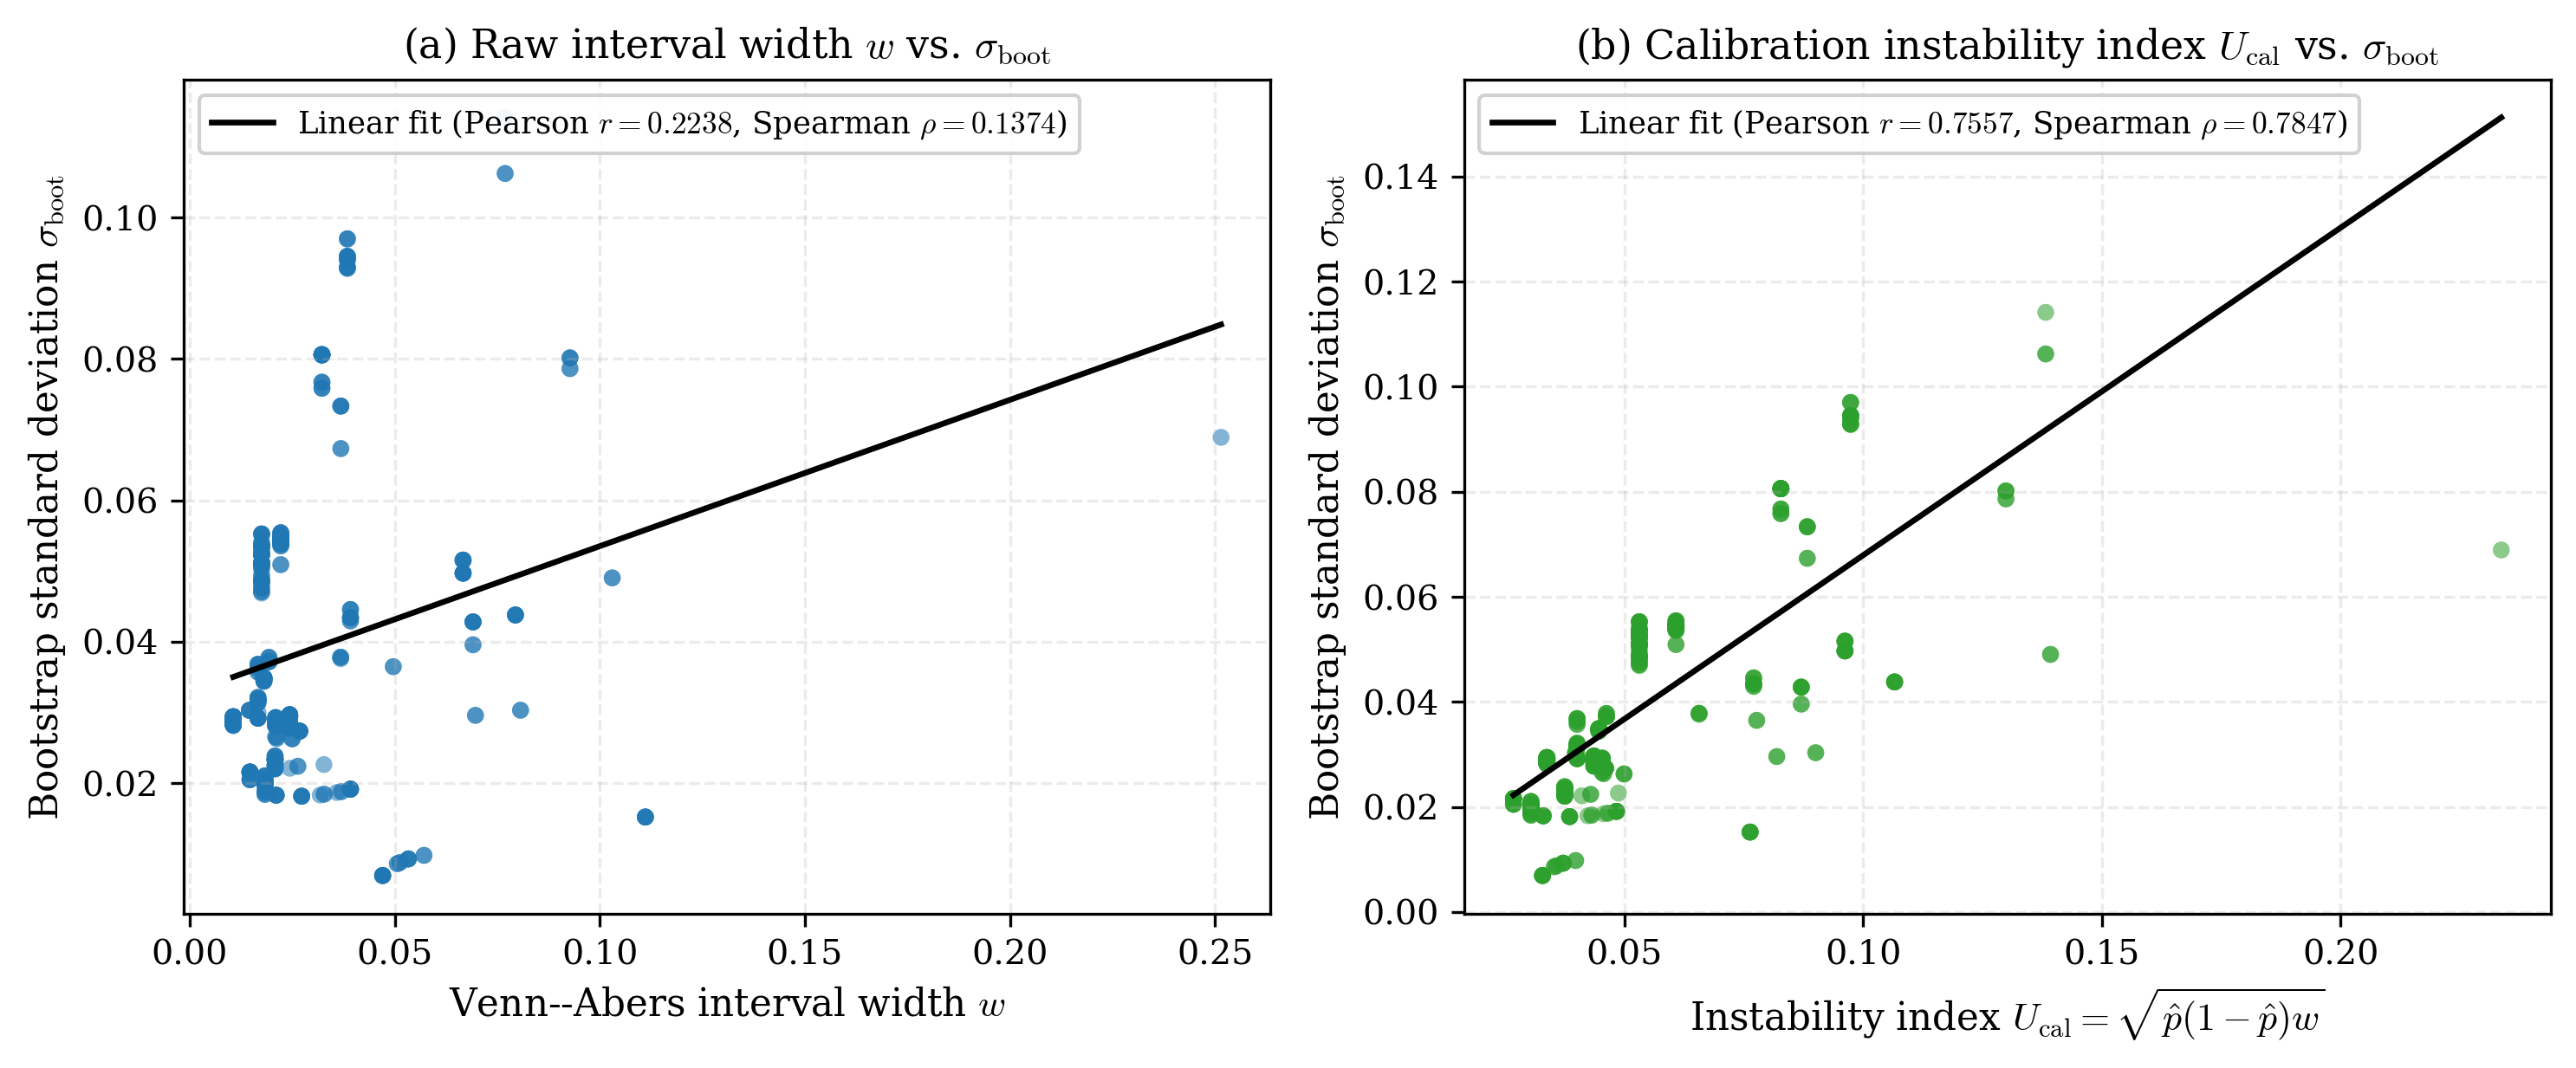
\includegraphics[width=0.92\textwidth]{width_vs_bootstrap_instability.png}
		\caption{Pointwise comparison of Venn--Abers interval width and probability-scale calibration instability in the classifier-based bootstrap experiment ($N_{\mathrm{cal}}=500$, $M=200$ resamples). Panel~(a) compares raw width $w$ with bootstrap standard deviation $\sigma_{\text{boot}}$ (Pearson $r = \WidthPearson{}$, Spearman $\rho = \WidthSpearman{}$). Panel~(b) compares the calibration instability index $U_{\text{cal}}=\sqrt{\hat p(1-\hat p)w}$ with bootstrap standard deviation (Pearson $r = \UCalPearson{}$, Spearman $\rho = \UCalSpearman{}$). In a held-out multiplicative fit, the mean absolute error is reduced from $\WidthMAE{}$ for width to $\UCalMAE{}$ for $U_{\mathrm{cal}}$.}
		\label{fig:width_vs_bootstrap_instability}
	\end{figure}

	\subsection{Empirical Verification of Scaling Laws}
	
	We first check the sample-size rates in a simple classifier-free experiment. We generate $S\sim U(0,1)$ and $Y\mid S=s\sim\operatorname{Bernoulli}(0.2+0.6s)$, and evaluate a fixed interior score $s_0=0.5$ over increasing calibration sizes. The fitted log--log slope of mean width is $\IdealWidthSlope{}$ (95\% CI $[\IdealWidthCILow{},\IdealWidthCIHigh{}]$), compared with the predicted $-2/3$. The standard deviation of the calibrated midpoint across Monte Carlo calibration samples has slope $\IdealSDSlope{}$ (95\% CI $[\IdealSDCILow{},\IdealSDCIHigh{}]$), while $U_{\mathrm{cal}}$ has slope $\IdealUCalSlope{}$ (95\% CI $[\IdealUCalCILow{},\IdealUCalCIHigh{}]$). All three confidence intervals contain their corresponding theoretical exponents, so in this controlled experiment the observed rates are consistent with the proposed $n^{-2/3}$ and $n^{-1/3}$ scalings.
	
\begin{figure}[ht]
\centering
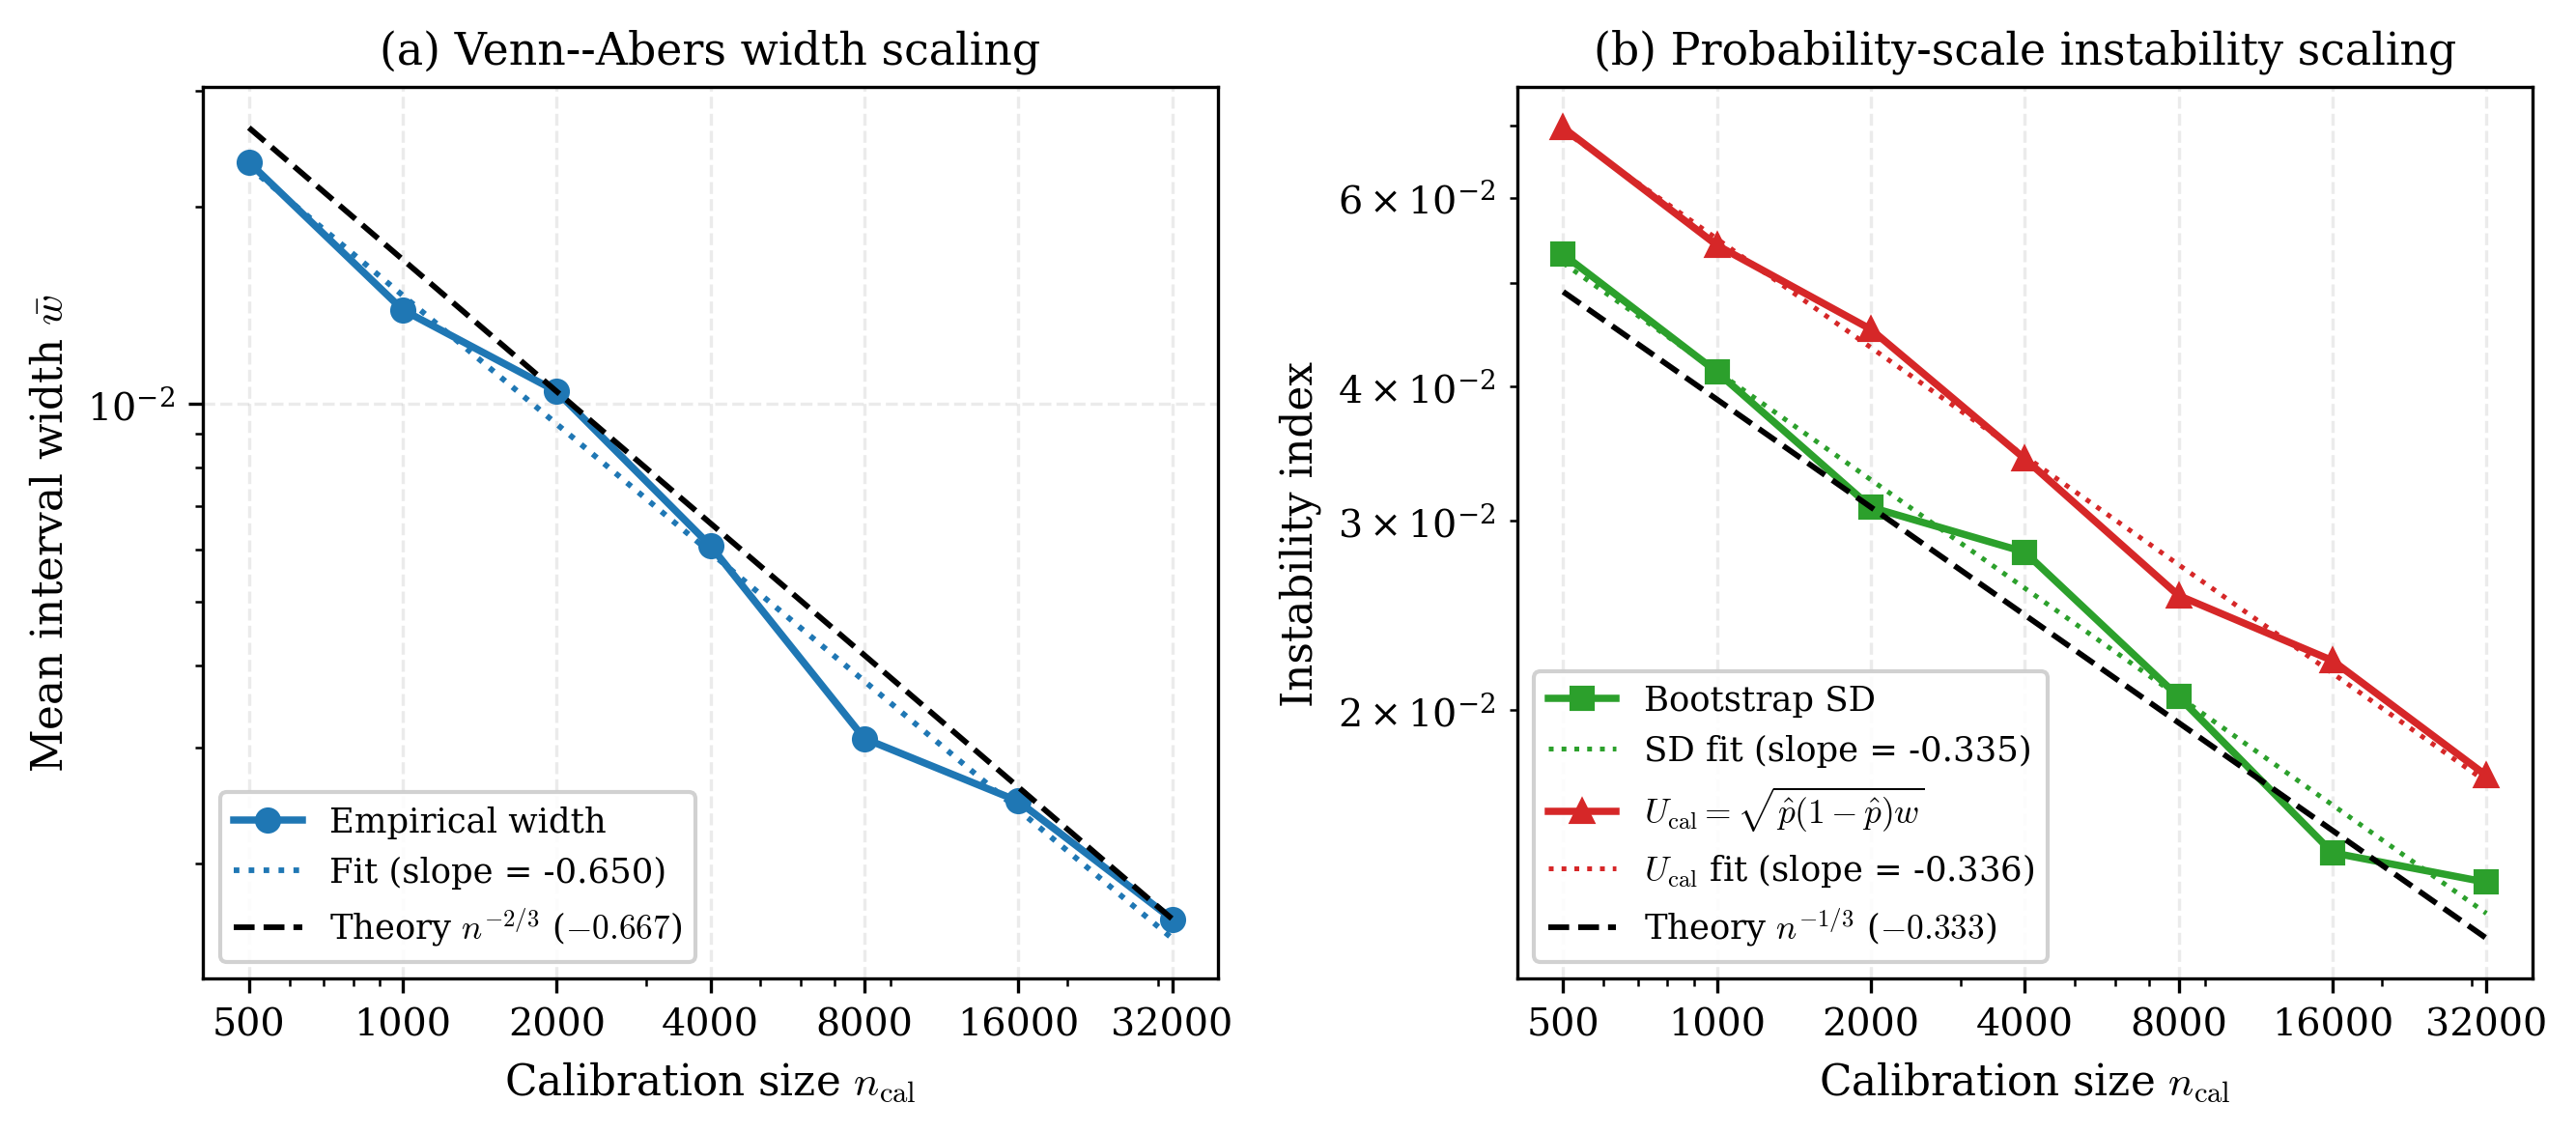
\includegraphics[width=0.9\textwidth]{idealised_scaling_laws.png}
\caption{Idealised scaling of Venn--Abers interval width and probability-scale calibration instability. Panel (a) shows the mean interval width as a function of calibration size, together with the predicted $n^{-2/3}$ reference rate. Panel (b) shows the bootstrap standard deviation of the calibrated probability and $U_{\mathrm{cal}}=\sqrt{\hat p(1-\hat p)w}$, together with the predicted $n^{-1/3}$ reference rate. The fitted slopes are $\IdealWidthSlope{}$ for width, $\IdealSDSlope{}$ for the standard deviation of the calibrated midpoint, and $\IdealUCalSlope{}$ for $U_{\mathrm{cal}}$.}
\label{fig:idealised_scaling}
\end{figure}
	
	We next test the local density, ambiguity, and slope exponents in a controlled multivariate design. At moderate sample sizes the estimated coefficients have the predicted signs but are attenuated relative to their asymptotic values. We therefore repeat the experiment over $n_{\mathrm{cal}}\in\{500,1000,2000,4000,8000,16000,32000\}$, covering four density regimes and six probability curves. For each sample size we fit
	\begin{equation}
		\log w
		=
		\alpha
		+\beta_\rho(n)\log f
		+\beta_v(n)\log[\theta(1-\theta)]
		+\beta_s(n)\log|\theta'|
		+\epsilon.
		\label{eq:empirical_exponent_regression}
	\end{equation}
	
\begin{table}[htbp]
\centering
\small
\setlength{\tabcolsep}{2.5pt}
\caption{Finite-sample estimates of the local scaling exponents as the calibration sample increases. The theoretical targets are $-2/3$ for local density, $-1/3$ for Bernoulli ambiguity, and $+2/3$ for local slope. Discrepancy from theoretical values attenuates substantially as $n_{\mathrm{cal}}$ increases.}
\label{tab:exponent_convergence}
\begin{tabular}{rccccc}
\toprule
$n_{\mathrm{cal}}$ & $\hat\beta_\rho$ [95\% CI] & $\hat\beta_v$ [95\% CI] & $\hat\beta_s$ [95\% CI] & Mean Abs.\ Error & $R^2$ \\
\midrule
500 & -0.438 [-0.465, -0.411] & -0.308 [-0.358, -0.255] & +0.635 [+0.576, +0.696] & 0.095 & 0.367 \\
1000 & -0.554 [-0.579, -0.530] & -0.310 [-0.360, -0.256] & +0.665 [+0.600, +0.726] & 0.046 & 0.465 \\
2000 & -0.519 [-0.551, -0.487] & -0.296 [-0.358, -0.238] & +0.670 [+0.598, +0.743] & 0.063 & 0.440 \\
4000 & -0.537 [-0.568, -0.507] & -0.325 [-0.390, -0.261] & +0.661 [+0.585, +0.742] & 0.048 & 0.433 \\
8000 & -0.583 [-0.626, -0.544] & -0.338 [-0.416, -0.260] & +0.650 [+0.555, +0.747] & 0.035 & 0.445 \\
16000 & -0.652 [-0.693, -0.611] & -0.398 [-0.486, -0.310] & +0.754 [+0.643, +0.868] & 0.055 & 0.495 \\
32000 & -0.672 [-0.729, -0.622] & -0.299 [-0.409, -0.196] & +0.663 [+0.524, +0.808] & 0.014 & 0.540 \\
\bottomrule
\end{tabular}
\end{table}

	
	The coefficients are quite far from the theoretical values for the smaller calibration samples, but the gap reduces as the sample becomes larger. At $n=500$, the three local coefficients are approximately $(-0.438,-0.308,+0.635)$ for density, ambiguity, and slope. By $n=8000$ they are approximately $(-0.583,-0.338,+0.650)$, and at $n=16000$ they are $(-0.652,-0.398,+0.754)$. The theoretical targets $(-2/3,-1/3,+2/3)$ lie inside the empirical confidence intervals at the larger calibration sizes. At $n=32000$, the estimates reach $(-0.672,-0.299,+0.663)$, with a mean absolute discrepancy of only $0.014$ across all three exponents, and all theoretical targets remain inside the corresponding empirical confidence intervals.
	
	The mean absolute discrepancy from the theoretical exponents decreases with $\log n$ at slope $-0.0130$ ($p=0.0396$), with the density discrepancy showing a particularly strong downward trend (slope $-0.0479$, $p=0.0031$). Across all calibration sizes ($n \in [500, 32{,}000]$), the pooled regression is
	\begin{equation}
		\log w
		=
		-0.6701\log n
		-0.5378\log f
		-0.3191\log[\theta(1-\theta)]
		+0.6640\log|\theta'|
		+\text{constant},
		\label{eq:pooled_w2}
	\end{equation}
	with $R^2=0.6796$. The pooled local coefficients remain attenuated because this regression combines the small-$n$ and large-$n$ regimes. The results therefore support the proposed direction of the scaling law, with the finite-sample coefficients getting closer to the theoretical values as the calibration sample increases.
	
\begin{figure}[ht]
\centering
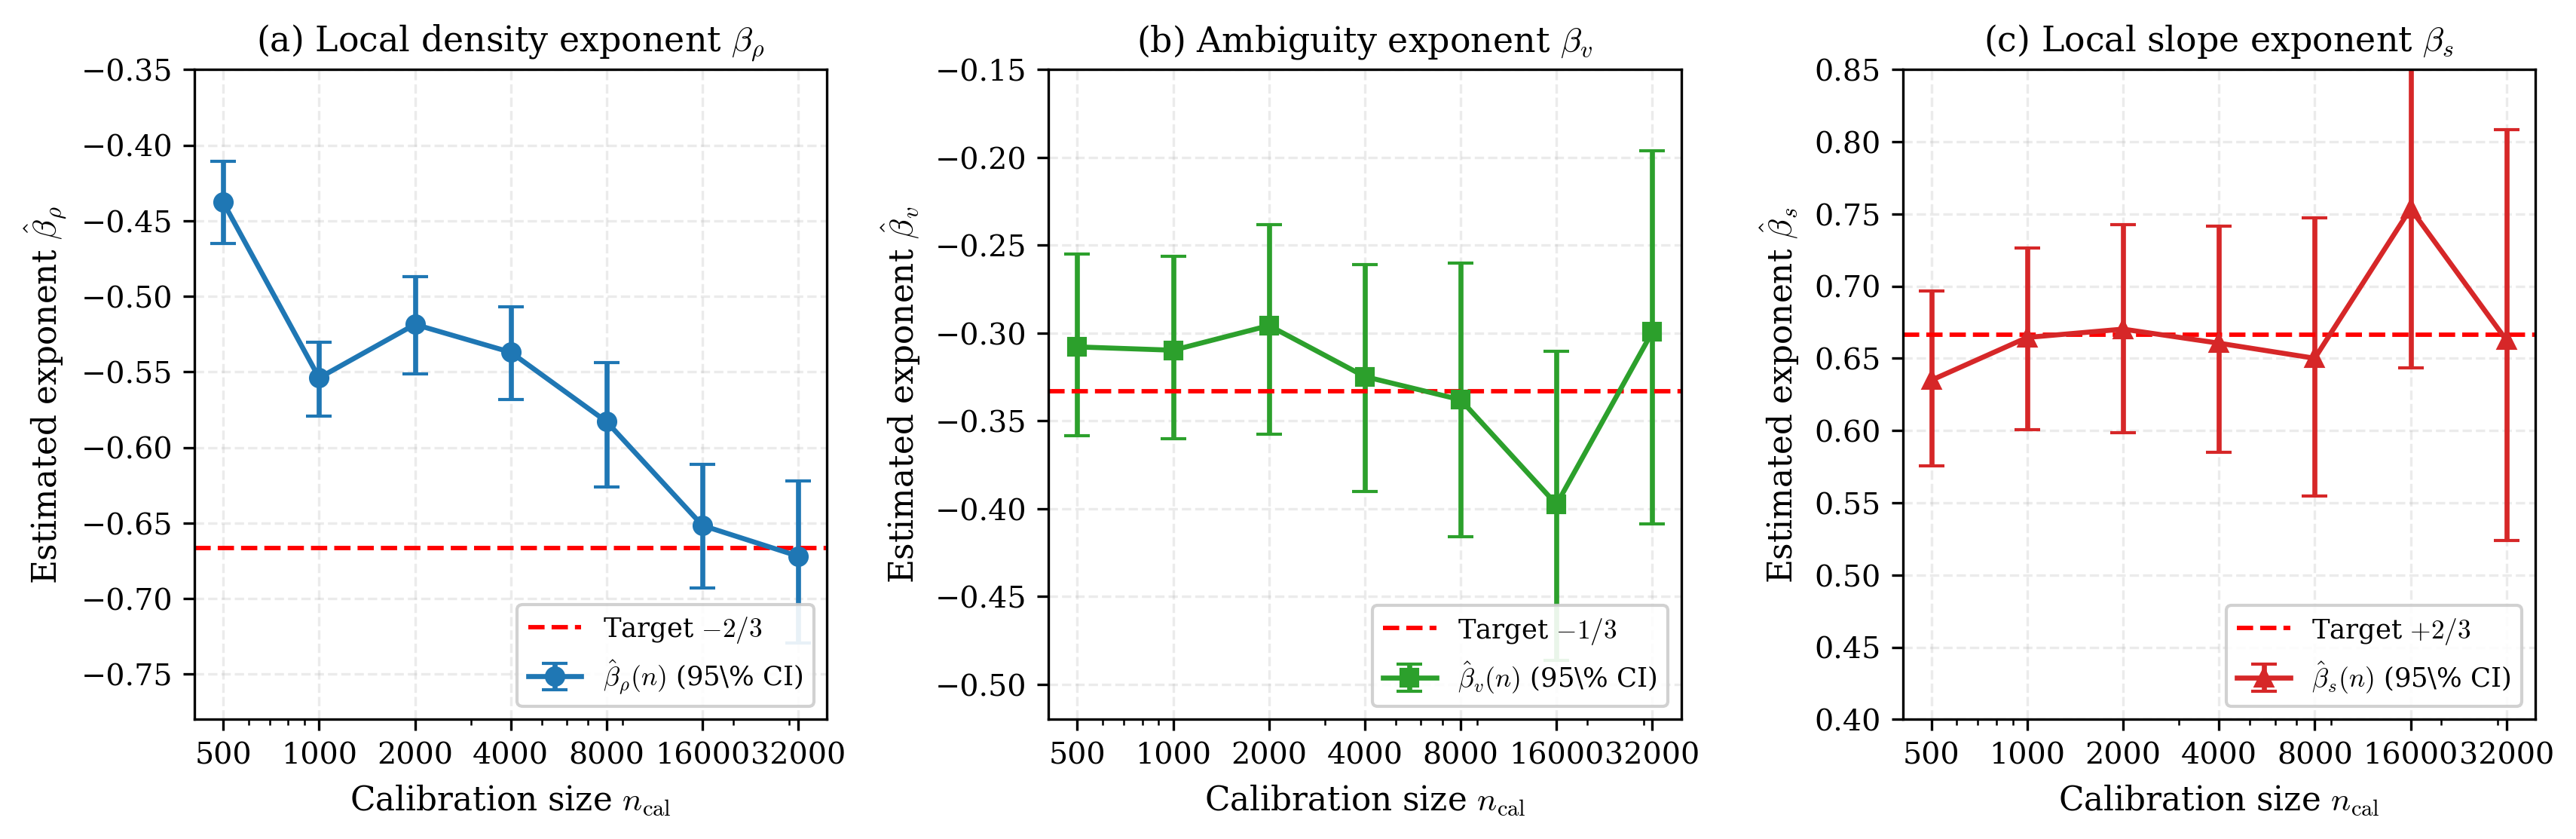
\includegraphics[width=0.95\textwidth]{w2_exponent_convergence.png}
\caption{Estimated local density, ambiguity, and slope exponents over increasing calibration sample sizes. Points show fitted coefficients and error bars show 95\% confidence intervals. Dashed horizontal lines denote the theoretical targets $-2/3$, $-1/3$, and $+2/3$. The initially attenuated coefficients move substantially toward the proposed asymptotic values as the calibration sample increases, although the progression is not monotonic at the largest sample size.}
\label{fig:exponent_convergence}
\end{figure}
	
	\subsection{Empirical Verification of Non-Monotonicity and Transformation Invariance}
	\label{subsec:non_monotonic_results}
	
	We next evaluate VAPs under two non-linear regimes: strictly increasing but non-linear transformations of the scores, and local violations of monotonicity.
	
	\paragraph{1. Monotonic Score Invariance:}
	We empirically verify the theoretical claim that VAP calibration outputs depend only on the rank ordering of the base model's predictions. We generate a calibration set with scores $s \in [0, 1]$ and true probabilities $\theta(s) = s^2$. We then apply Venn--Abers calibration at a test score $s_{\text{test}} = 0.5$ using three score transformations: (i) the original scores $s$, (ii) a quadratic transform $s^2$, and (iii) an exponential transform $\exp(s)$. 
	Under all three transformations, the calibrated outputs at the corresponding test points are identical: $p_0 = 0.200000$, $p_1 = 0.212500$, and interval width $w = 0.012500$. This shows that, in this experiment, strictly increasing transformations of the base classifier's scores leave the calibrated intervals unchanged.
	
	\paragraph{2. Density Scaling under Non-Monotonicity:}
	Next, we study how the interval width scaling law varies when the monotonicity assumption is violated. We run calibration over sizes $N \in [100, 3200]$ across four distinct slope regimes at a fixed test point $s_{\text{test}} = 0.0$ (which corresponds to the center of the score support where the designed local extrema and flat inflection points are situated):
	\begin{itemize}
		\item \textbf{Regime A (Standard Monotonic):} $\theta(s) = 0.5 + 0.3 s$ (positive slope $\theta' = 0.3$). The empirical exponent of width vs $N$ is $\NonMonoRegimeASlope{}$, matching the theoretical exponent of $-2/3 \approx -0.667$.
		\item \textbf{Regime B (Monotonicity-Violating):} $\theta(s) = 0.5 - 0.3 s$ (negative slope $\theta' = -0.3$). Because the probability decreases, the PAV algorithm merges all points into a single block containing a non-vanishing fraction of the $N$ calibration observations. The empirical exponent is $\NonMonoRegimeBSlope{}$, matching the theoretical value of $-1.000$.
		\item \textbf{Regime C (Local Extremum with Violation):} $\theta(s) = 0.5 - 0.4 s^2$ on $s \in [-1, 1]$ (parabolic middle peak, $\theta'(0) = 0$). Here, the right half ($s > 0$) decreases, violating monotonicity and forcing a macroscopic merge. The peak at $s=0.0$ is merged into this violating block, and the empirical exponent is $\NonMonoRegimeCSlope{}$, aligning with the $-1.000$ limit.
		\item \textbf{Regime D (Order-Two Flat/Kink Regime):} $\theta(s) = 0.5 + 0.4 s^2 \operatorname{sign}(s)$ on $s \in [-1, 1]$, equivalently $\theta(s) = 0.5 + 0.4 s|s|$. The function is $C^1$ (continuously differentiable) with local change of order $|s|^2$, but $\theta'$ has a kink at the origin, so $\theta$ is not twice differentiable there. Equation~\ref{eq:general_order_scaling} with $\alpha=2$ therefore predicts the $-4/5$ sample-size exponent. The empirical exponent is $\NonMonoRegimeDSlope{}$, close to $-4/5=-0.800$. A smooth monotone cubic flat point would instead correspond to $\alpha=3$ and the $-6/7$ rate.
	\end{itemize}
	These scaling regimes are shown in Figure~\ref{fig:non_monotonic_scaling_laws}.
	
	\begin{figure}[ht]
		\centering
		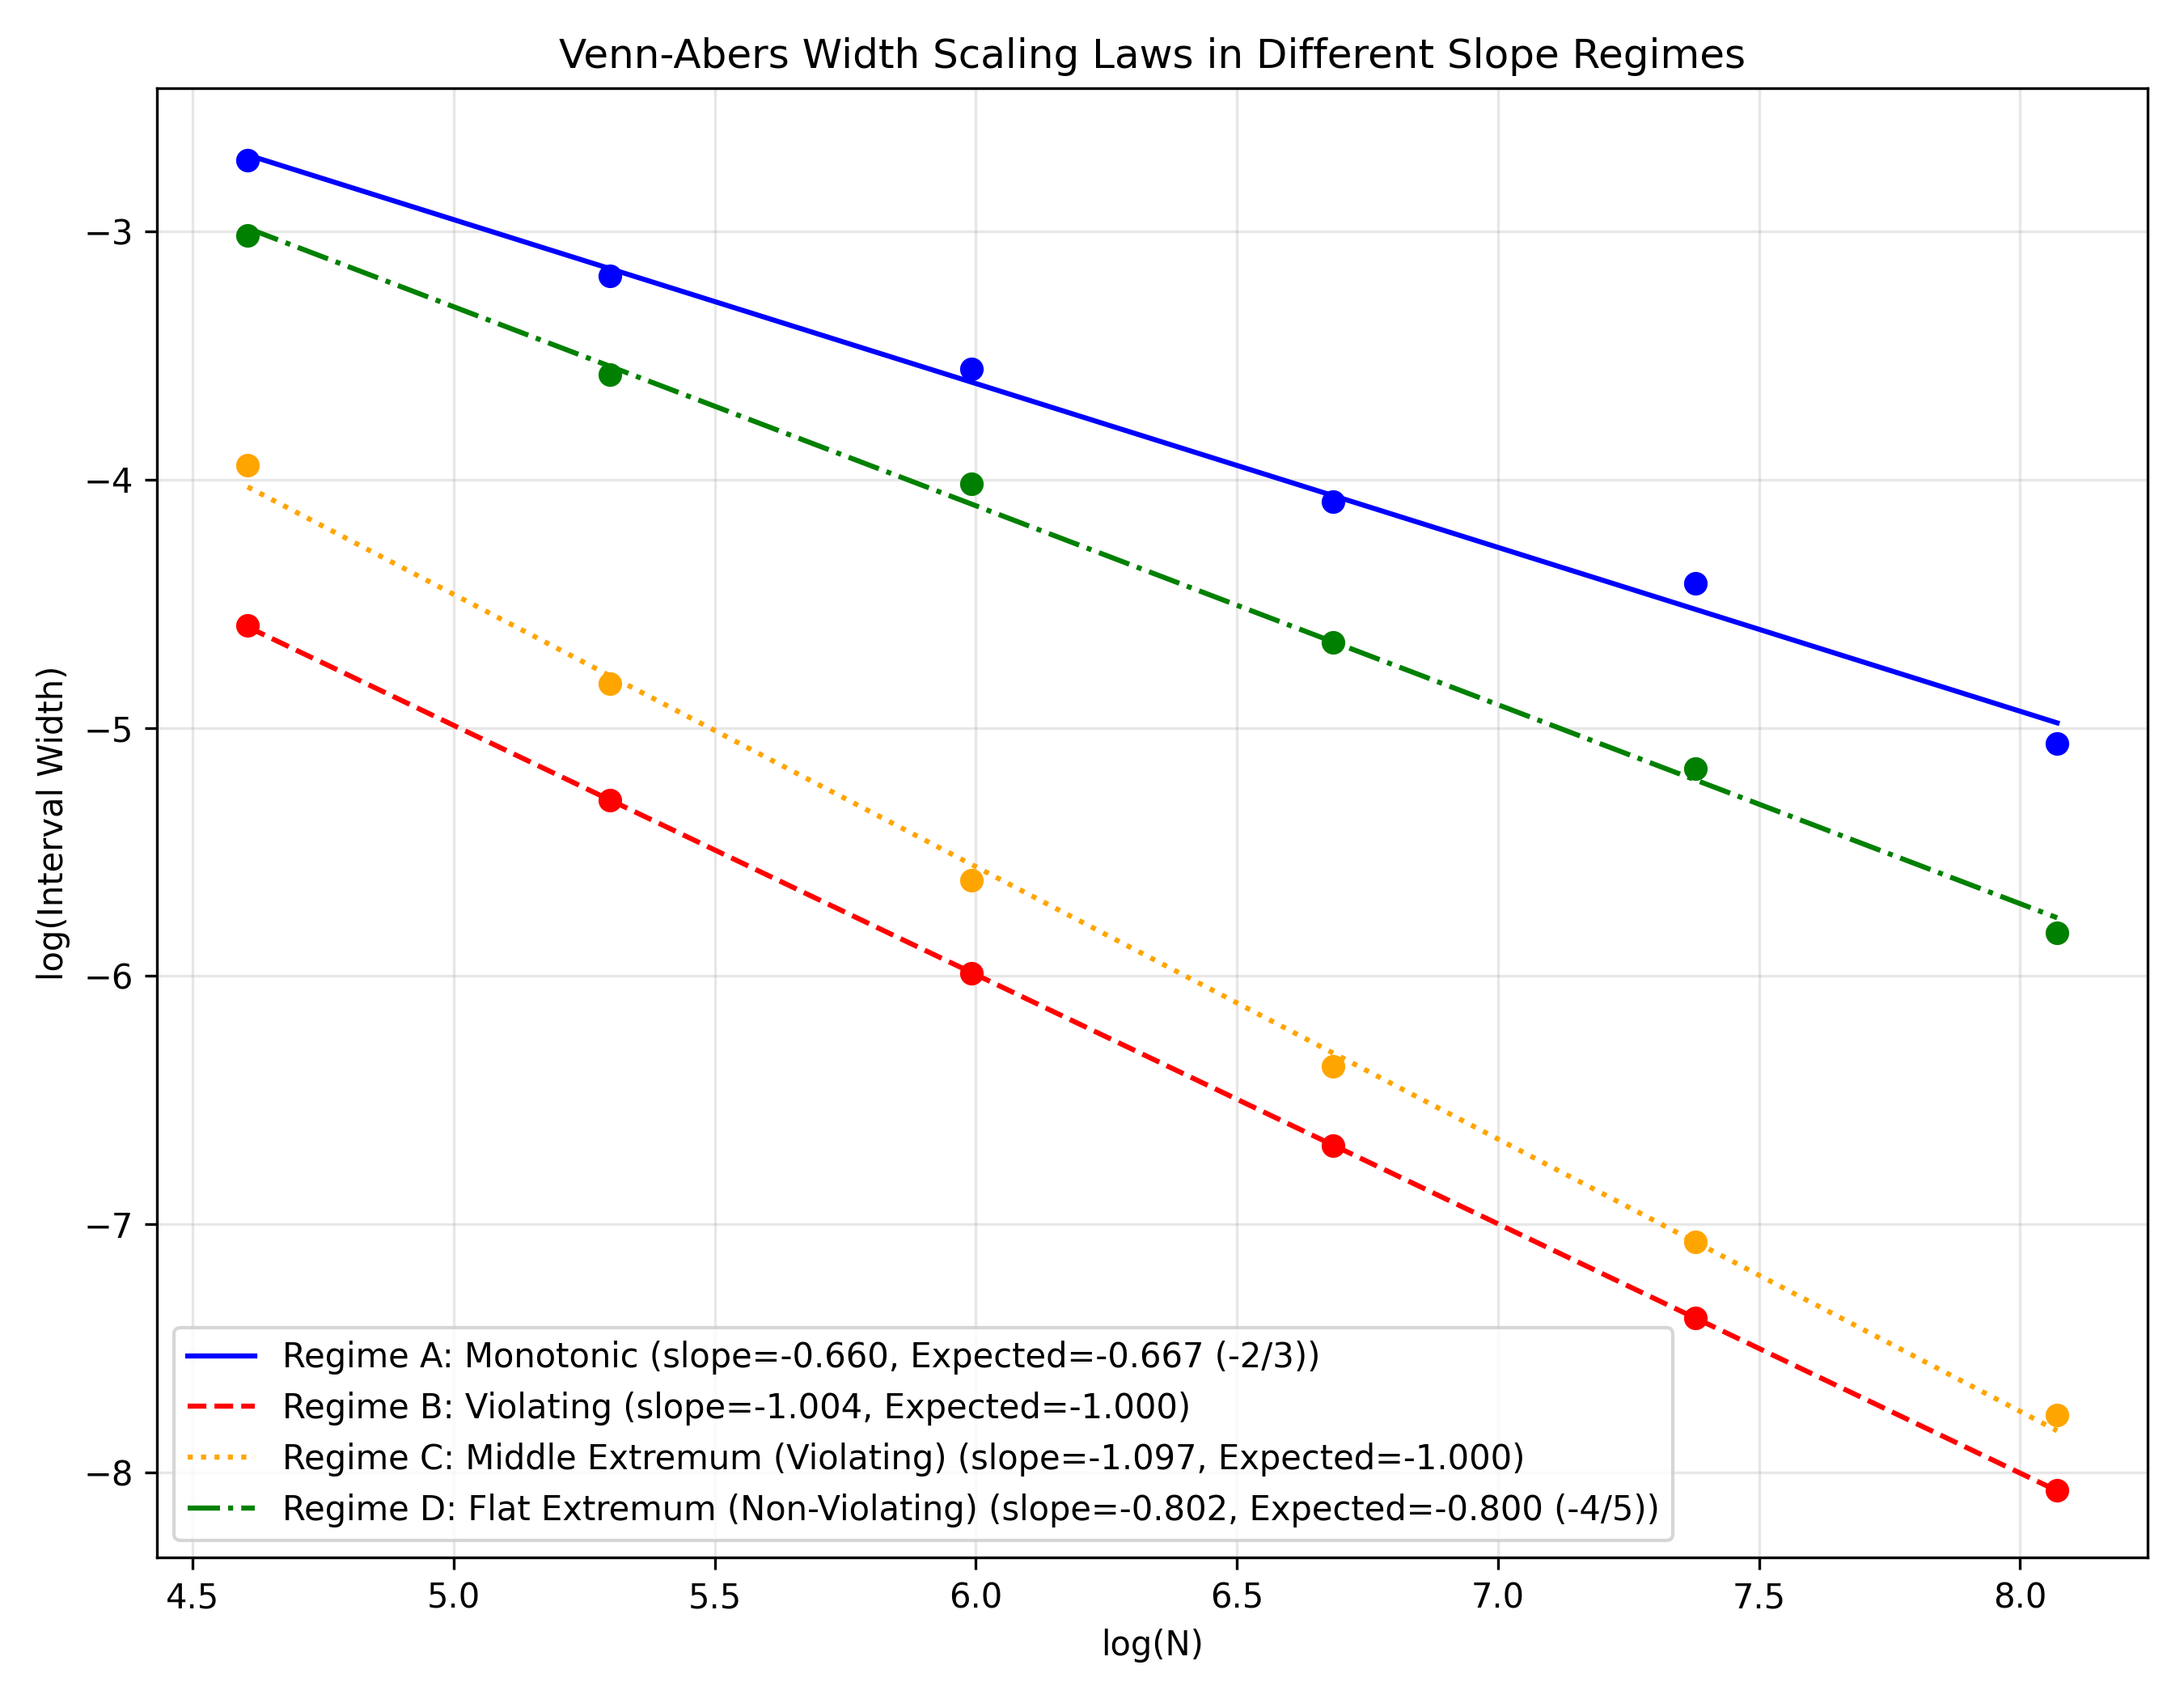
\includegraphics[width=0.75\textwidth]{non_monotonic_scaling_laws.png}
		\caption{Log-log plots of Venn--Abers interval width vs. calibration set size for standard monotonic (Regime A), monotonicity-violating (Regime B), middle-peak violation (Regime C), and order-two flat/kink (Regime D) setups. The empirical exponents are close to the corresponding predicted rates of $-2/3$, $-1$, $-1$, and $-4/5$.}
		\label{fig:non_monotonic_scaling_laws}
	\end{figure}
	
	\subsection{Ambiguity vs. Instability in a Crowd Annotation Simulation}
	\label{subsec:cifar_results}
	
	We also compare width with label ambiguity in a simulated crowd-annotation problem based on the structure of CIFAR-10H. We use a simulation rather than the original labels because the underlying class probabilities and score distributions are then known, and because repeated bootstrap fitting is much cheaper. The experiment is therefore intended as a controlled ambiguity test rather than as a CIFAR-10H benchmark. Specifically, we generate synthetic feature embeddings $X \in \mathbb{R}^{2000 \times 64}$ and multiclass logits to define a 10-class dataset. The soft label for any given class is computed directly as the softmax-normalized probability of the multiclass logits, representing the infinite-annotator limit of annotator agreement. The binary tasks are defined using a one-vs-rest mapping. Under this configuration, we can explicitly compare the VAP interval width against:
	\begin{enumerate}
		\item \textbf{Bootstrap Instability}: The empirical standard deviation of the calibrated predictions across $M=100$ bootstrap draws of the calibration set.
		\item \textbf{Annotator Disagreement}: The probability that two independently sampled annotators assign different binary labels, equal to $2p(1-p)$ for binary target probability $p$. The underlying Bernoulli label variance is $p(1-p)$.
		\item \textbf{Annotator Entropy}: The Shannon entropy of the annotator labels.
	\end{enumerate}
	
	We fit a base classification model (\texttt{HistGradientBoostingClassifier}) on the training portion of the generated feature embeddings to predict one-vs-rest class probabilities, and calibrate its predictions on the test set using a Venn--Abers predictor fitted on the calibration set. We then compute the macro-averaged Pearson and Spearman correlation coefficients of the VAP interval width against each of the three quantities across all ten classes.
	
	\begin{table}[htbp]
\centering
\caption{Macro-averaged Pearson and Spearman correlations of Venn--Abers interval width with bootstrap instability, annotator disagreement, and annotator entropy in the synthetic CIFAR-10H-inspired crowd-annotation experiment.}
\label{tab:cifar_correlations}
\begin{tabular}{lcc}
\toprule
Quantity & Pearson Correlation & Spearman Correlation \\
\midrule
Bootstrap Instability & 0.5000 & 0.5279 \\
Annotator Disagreement & 0.0007 & 0.0007 \\
Annotator Entropy & 0.0013 & 0.0007 \\
\bottomrule
\end{tabular}
\end{table}

	
	Table~\ref{tab:cifar_correlations} gives the macro-averaged correlations. The pattern is different for calibration instability and for the two ambiguity measures:
	\begin{itemize}
		\item The VAP interval width has a positive correlation with \textbf{Bootstrap Instability} (Pearson $\approx \CifarBootPearson{}$, Spearman $\approx \CifarBootSpearman{}$). This suggests that wider intervals tend to occur for test points for which the calibrated probability is more sensitive to the particular finite calibration sample drawn.
		\item Conversely, the VAP interval width has essentially zero correlation with \textbf{Annotator Disagreement} (Pearson $\approx \CifarDisPearson{}$, Spearman $\approx \CifarDisSpearman{}$) and \textbf{Annotator Entropy} (Pearson $\approx \CifarEntPearson{}$, Spearman $\approx \CifarEntSpearman{}$). 
	\end{itemize}
	In this experiment width is therefore related to finite-sample calibration sensitivity, while there is almost no relationship with either annotator disagreement or entropy.

	\subsection{Controlled Local Support Thinning on Real Tabular Datasets}
	\label{subsec:real_data_results}

	To directly test the calibration-support interpretation in a non-synthetic environment, we examine the response of Venn--Abers interval width and calibration instability under controlled thinning of local calibration support across UCI Adult, UCI Bank Marketing, and UCI Spambase.

	Figure~\ref{fig:real_data_local_support} presents the principal experimental results.

	\begin{figure}[htbp]
		\centering
		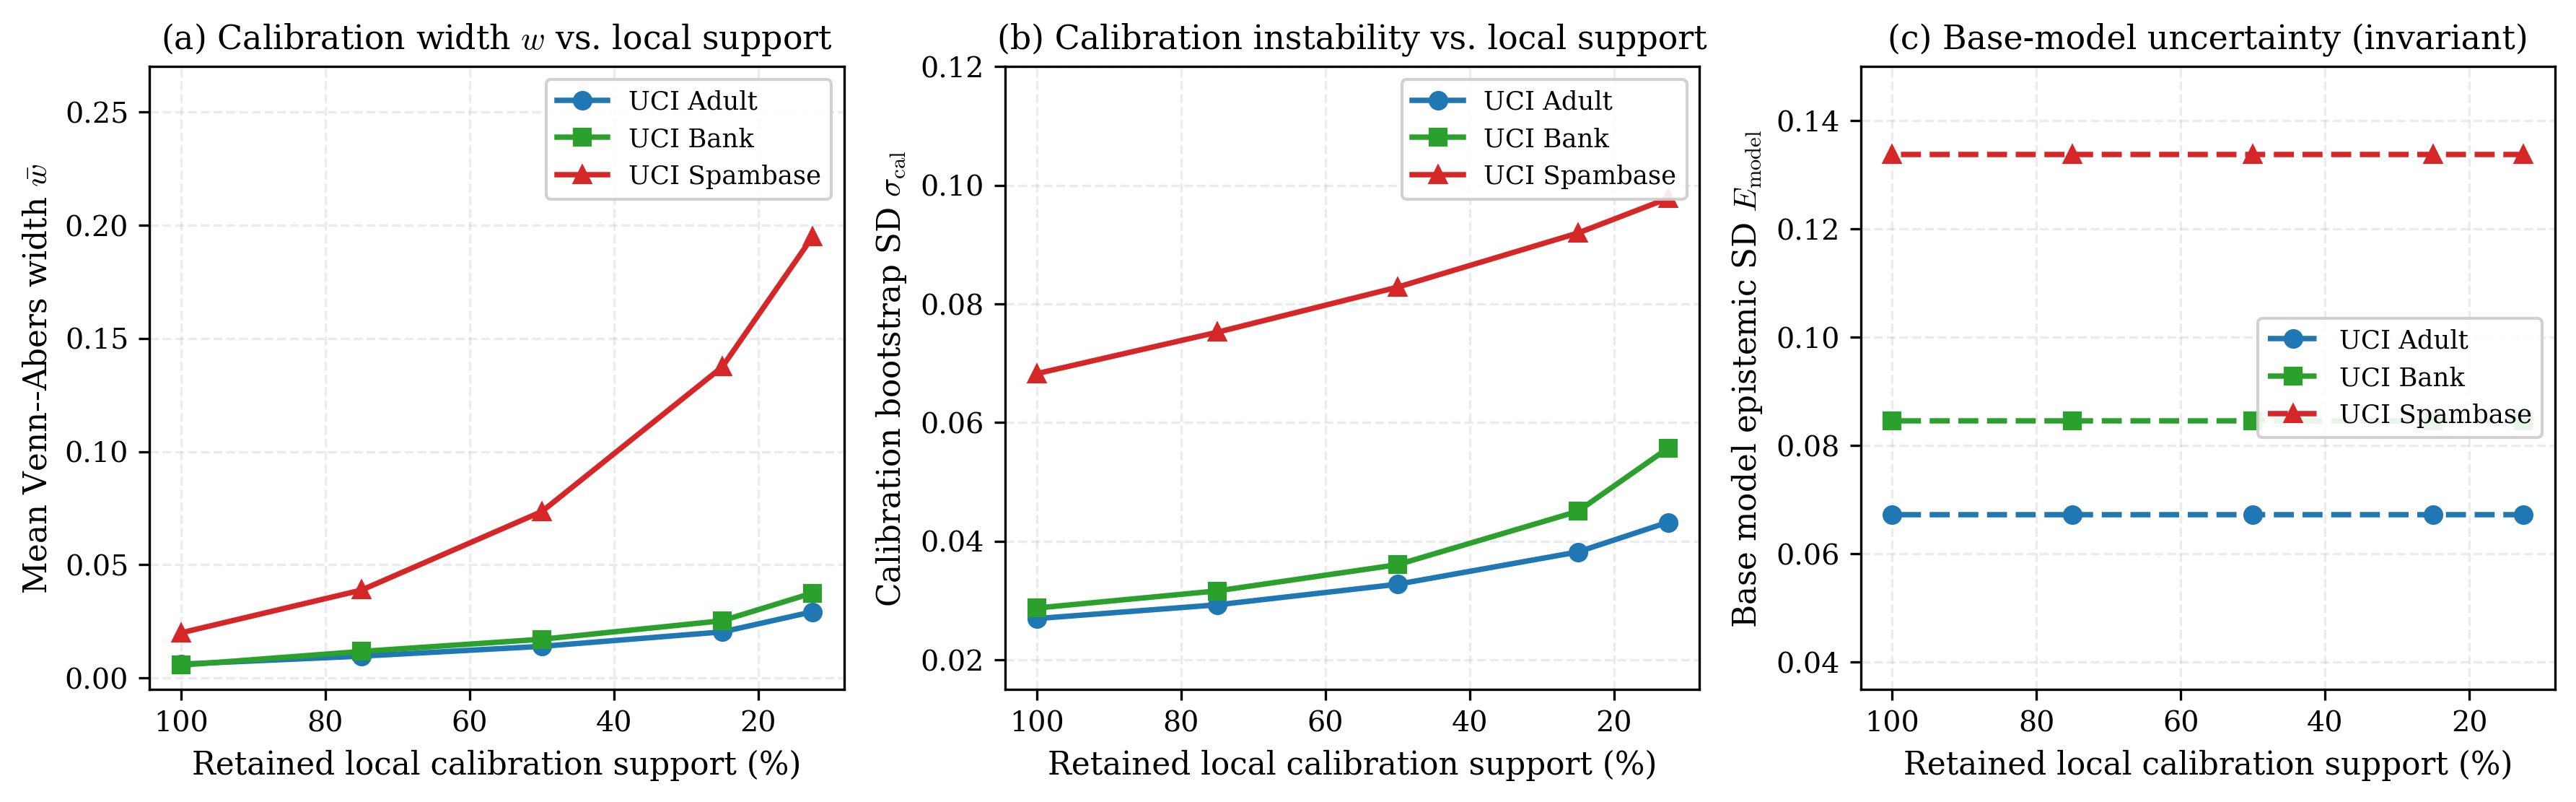
\includegraphics[width=0.98\textwidth]{real_data_local_support.png}
		\caption{Controlled local calibration-support thinning on real tabular datasets (UCI Adult, UCI Bank Marketing, UCI Spambase). Panel~(a) shows mean Venn--Abers interval width $\bar{w}$ as local calibration support in the 10\% score rank neighbourhood is thinned from 100\% down to 12.5\%. Panel~(b) shows empirical calibration bootstrap standard deviation $\sigma_{\mathrm{cal}}$. Panel~(c) shows base-model epistemic uncertainty $E_{\mathrm{model}}$, which is unchanged by construction because the base classifier and training data are held fixed while local calibration support is manipulated.}
		\label{fig:real_data_local_support}
	\end{figure}

	The empirical results provide direct support for the theoretical framework:
	\begin{enumerate}
		\item \textbf{Venn--Abers Width Responds Monotonically to Calibration Support:} As the retained fraction of calibration observations in the local neighbourhood decreases from 100\% to 12.5\%, the mean Venn--Abers width increases monotonically across all three datasets (Panel~a). On UCI Adult, mean width rises from $\AdultWidthStart{}$ to $\AdultWidthEnd{}$; on UCI Bank Marketing, from $\BankWidthStart{}$ to $\BankWidthEnd{}$; and on UCI Spambase, from $\SpambaseWidthStart{}$ to $\SpambaseWidthEnd{}$.
		\item \textbf{Calibration Instability Strongly Corresponds to Width:} As local calibration support is removed, the empirical bootstrap standard deviation of the calibrated probabilities ($\sigma_{\mathrm{cal}}$) exhibits an identical upward progression (Panel~b), rising from $\AdultSigmaCalStart{}$ to $\AdultSigmaCalEnd{}$ on Adult, from $\BankSigmaCalStart{}$ to $\BankSigmaCalEnd{}$ on Bank Marketing, and from $\SpambaseSigmaCalStart{}$ to $\SpambaseSigmaCalEnd{}$ on Spambase.
		\item \textbf{Base-Model Uncertainty Control:} Panel~(c) displays the base-model epistemic uncertainty $E_{\mathrm{model}}(x)$. Because the base model and training data are held fixed, estimated base-model epistemic uncertainty is unchanged by construction ($\AdultEModel{}$ on Adult, $\BankEModel{}$ on Bank, and $\SpambaseEModel{}$ on Spambase). This isolates the response of width to changes in calibration support, verifying that the empirical inflation in width and calibration instability is not confounded by base-model variation.
	\end{enumerate}

	\paragraph{Reverse Intervention: Manipulating Training Support.}
	In the reverse intervention, we hold the calibration set fixed and subsample the training partition from 100\% down to 25\%. As shown in Figure~\ref{fig:training_support_epistemic}, decreasing training support systematically inflates base-model epistemic uncertainty $E_{\mathrm{model}}$ (Panel~a, increasing from $\AdultRevEModelStart{}$ to $\AdultRevEModelEnd{}$ on Adult, from $\BankRevEModelStart{}$ to $\BankRevEModelEnd{}$ on Bank, and from $\SpambaseRevEModelStart{}$ to $\SpambaseRevEModelEnd{}$ on Spambase). In contrast, Venn--Abers interval width changes much less on Adult (Panel~b, from $\AdultRevWidthStart{}$ to $\AdultRevWidthEnd{}$) and Bank (from $\BankRevWidthStart{}$ to $\BankRevWidthEnd{}$). A larger secondary change is visible on Spambase (from $\SpambaseRevWidthStart{}$ to $\SpambaseRevWidthEnd{}$), because retraining the base predictor changes the score function $g(x)$ and therefore the positions and ranking of the calibration scores even though the calibration instances themselves are fixed. These results are consistent with width being more directly sensitive to calibration support than to base-model training-set size.

	\begin{figure}[htbp]
		\centering
		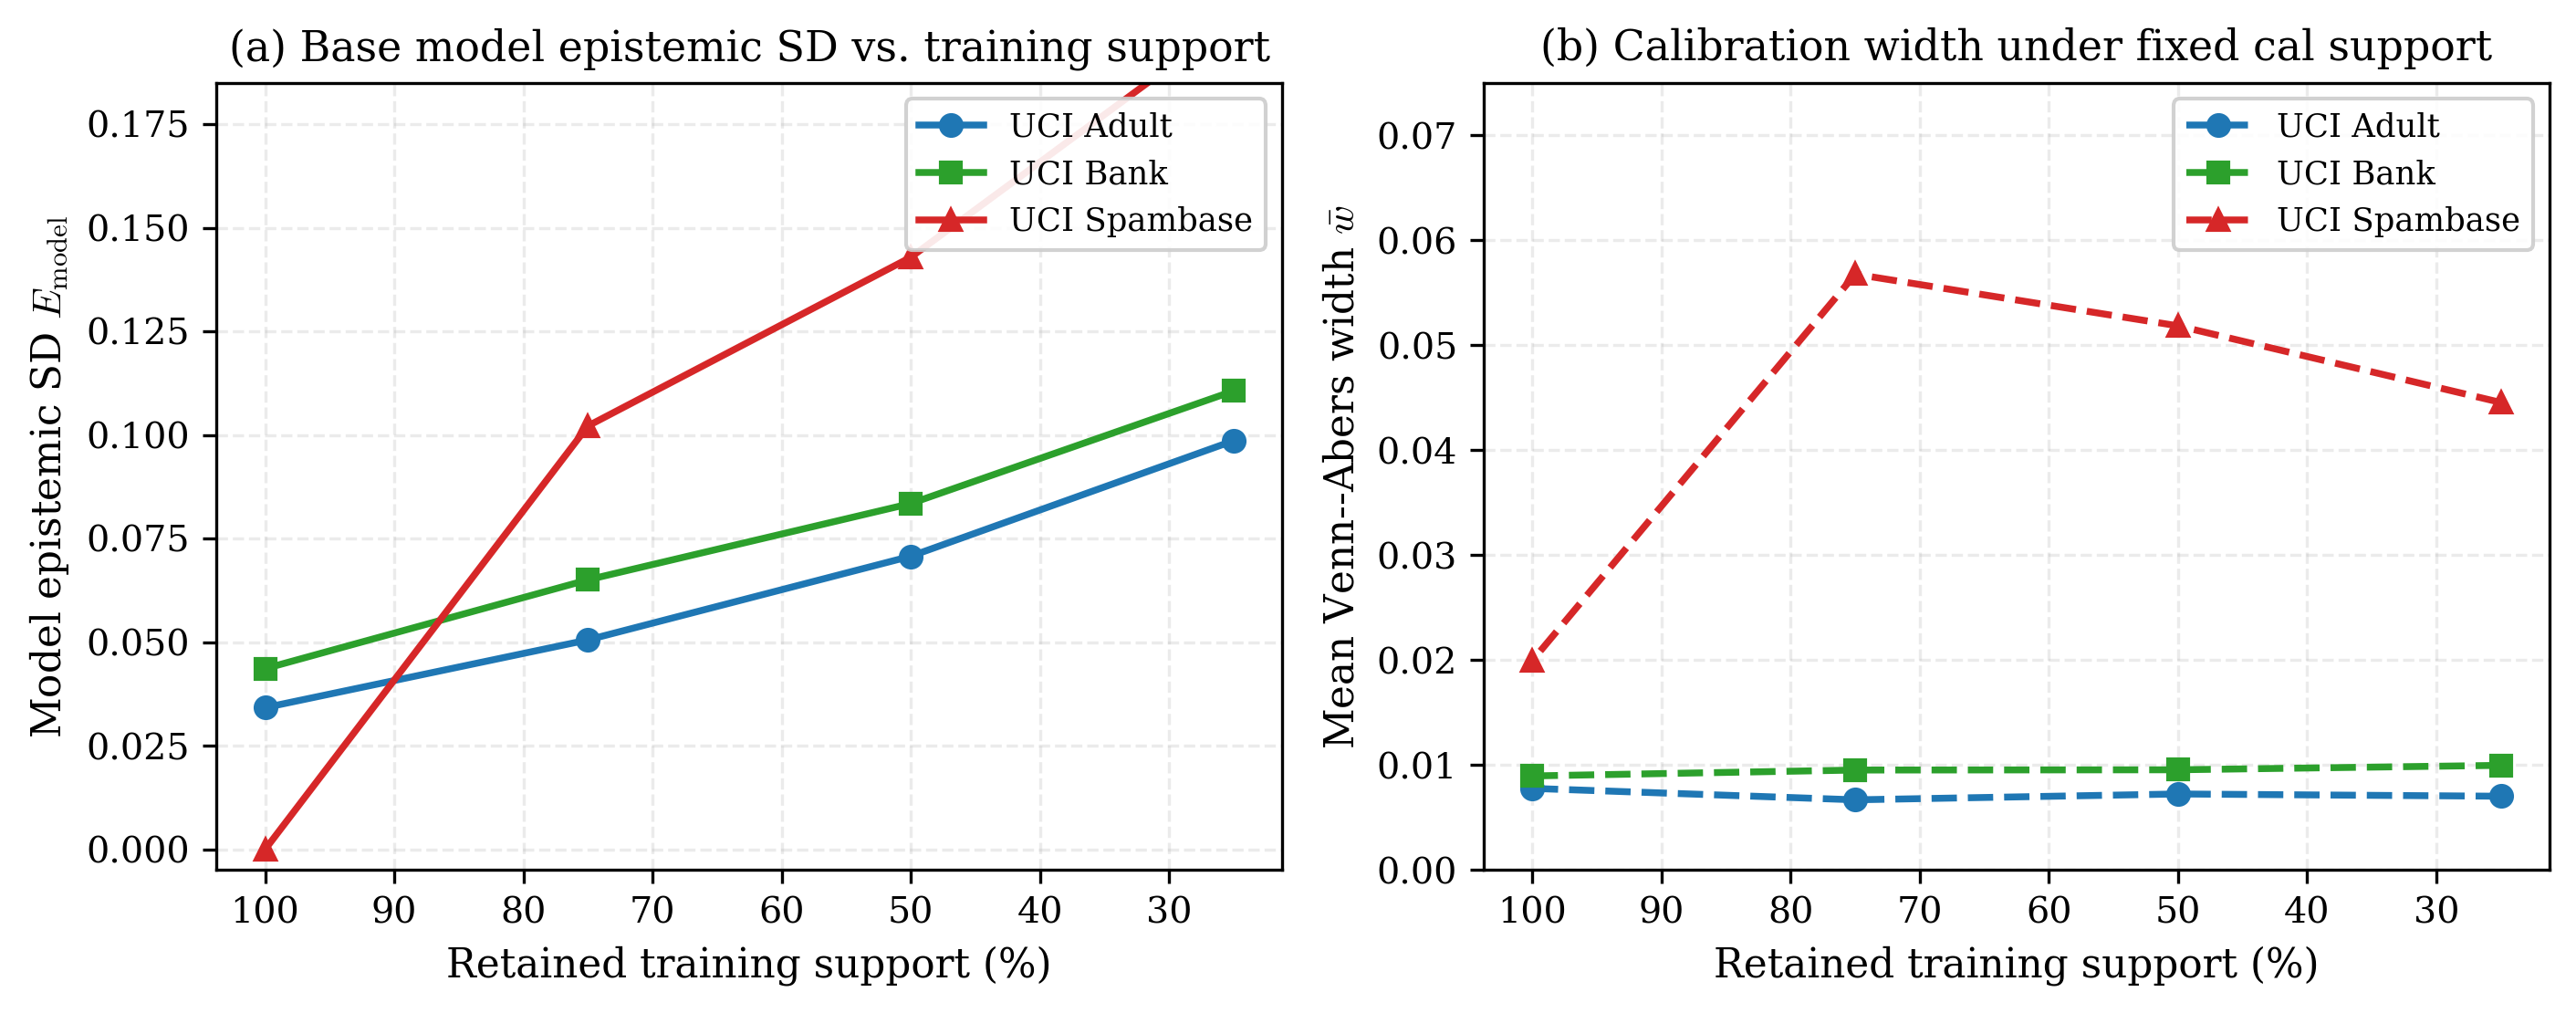
\includegraphics[width=0.88\textwidth]{training_support_epistemic.png}
		\caption{Reverse intervention altering base-model training support. Panel~(a) shows that reducing training support systematically increases base-model epistemic uncertainty $E_{\mathrm{model}}$. Panel~(b) demonstrates that Venn--Abers width is considerably less responsive to reduced training support than base-model bootstrap variability, particularly on Adult and Bank, with modest secondary variations attributable to score-geometry shifts under retraining.}
		\label{fig:training_support_epistemic}
	\end{figure}

	\paragraph{Quantitative Uncertainty Decomposition.}
	To evaluate whether Venn--Abers width provides calibration-specific information beyond outcome ambiguity and base-model uncertainty, we estimate pointwise calibration bootstrap instability $\sigma_{\mathrm{cal}}(x)$ on held-out test points and fit three nested regression specifications:
	\begin{align}
		\text{Model A: } &\sigma_{\mathrm{cal}}(x) = \alpha + \beta_A A(x) + \epsilon, \\
		\text{Model B: } &\sigma_{\mathrm{cal}}(x) = \alpha + \beta_A A(x) + \beta_E E_{\mathrm{model}}(x) + \epsilon, \\
		\text{Model C: } &\sigma_{\mathrm{cal}}(x) = \alpha + \beta_A A(x) + \beta_E E_{\mathrm{model}}(x) + \beta_w w(x) + \epsilon.
	\end{align}
	The comparative performance across 2,000 bootstrap resamples is summarized in Table~\ref{tab:real_data_nested}.

	\begin{table}[htbp]
\centering
\small
\caption{Held-out real-data comparison of calibration-instability models across three public tabular benchmarks ($N=500$ test points, $B_{\mathrm{cal}}=200$ resamples). Model A uses score-conditional outcome ambiguity $A(x)=\hat p(1-\hat p)$; Model B adds base-model epistemic uncertainty $E_{\mathrm{model}}(x)$; Model C adds Venn--Abers width $w(x)$. Across all datasets, Venn--Abers width provides an additional statistically detectable contribution to explaining calibration instability ($\Delta R^2$, 95\% bootstrap CI over 2,000 resamples), consistent with width capturing calibration-support information distinct from outcome ambiguity and base-model uncertainty.}
\label{tab:real_data_nested}
\begin{tabular}{llccc}
\toprule
Dataset & Model Specification & $R^2$ & MAE & RMSE \\
\midrule
\multirow{4}{*}{UCI Adult} & Model A: Ambiguity $A$ & 0.8525 & 0.0030 & 0.0042 \\
 & Model B: Ambiguity + $E_{\mathrm{model}}$ & 0.8559 & 0.0030 & 0.0041 \\
 & Model C: Ambiguity + $E_{\mathrm{model}}$ + Width $w$ & \textbf{0.9053} & \textbf{0.0023} & \textbf{0.0033} \\
 & $\Delta R^2$ (Model C $-$ Model B) & \multicolumn{3}{c}{+ 0.0494 [95\% CI: 0.0305, 0.0741]} \\
\midrule
\multirow{4}{*}{UCI Bank} & Model A: Ambiguity $A$ & 0.9178 & 0.0018 & 0.0030 \\
 & Model B: Ambiguity + $E_{\mathrm{model}}$ & 0.9186 & 0.0018 & 0.0030 \\
 & Model C: Ambiguity + $E_{\mathrm{model}}$ + Width $w$ & \textbf{0.9407} & \textbf{0.0015} & \textbf{0.0026} \\
 & $\Delta R^2$ (Model C $-$ Model B) & \multicolumn{3}{c}{+ 0.0222 [95\% CI: 0.0094, 0.0410]} \\
\midrule
\multirow{4}{*}{UCI Spambase} & Model A: Ambiguity $A$ & 0.9491 & 0.0030 & 0.0048 \\
 & Model B: Ambiguity + $E_{\mathrm{model}}$ & 0.9533 & 0.0027 & 0.0046 \\
 & Model C: Ambiguity + $E_{\mathrm{model}}$ + Width $w$ & \textbf{0.9544} & \textbf{0.0027} & \textbf{0.0045} \\
 & $\Delta R^2$ (Model C $-$ Model B) & \multicolumn{3}{c}{+ 0.0011 [95\% CI: 0.0000, 0.0037]} \\
\bottomrule
\end{tabular}
\end{table}


	Across all three datasets, Model~A (score-conditional outcome ambiguity alone) accounts for a large baseline fraction of calibration variability ($R^2$ of $\AdultModelARsq{}$ on Adult, $\BankModelARsq{}$ on Bank, and $\SpambaseModelARsq{}$ on Spambase). Adding base-model epistemic uncertainty (Model~B) produces modest improvements. Adding Venn--Abers width $w$ (Model~C) provides additional explanatory power across all three datasets: $\Delta R^2 = +\AdultDeltaRsq{}$ on Adult (95\% bootstrap CI $[\AdultDeltaRsqCILow{}, \AdultDeltaRsqCIHigh{}]$), $\Delta R^2 = +\BankDeltaRsq{}$ on Bank (95\% bootstrap CI $[\BankDeltaRsqCILow{}, \BankDeltaRsqCIHigh{}]$), and $\Delta R^2 = +\SpambaseDeltaRsq{}$ on Spambase (95\% bootstrap CI $[\SpambaseDeltaRsqCILow{}, \SpambaseDeltaRsqCIHigh{}]$). The bootstrap intervals exclude zero for all three datasets, with the Bank and Spambase lower endpoints closest to zero ($\BankDeltaRsqCILow{}$ and $\SpambaseDeltaRsqCILow{}$ respectively). These results are consistent with width containing calibration-support information not accounted for by outcome ambiguity or the base-model bootstrap measure.

	% ============================================================
	\section{Comparison with Related Calibration Methods}
	\label{sec:alternatives}

	For comparison, we also look at the sampling variation of three standard post-hoc calibration methods: Isotonic Regression (IR), Platt Scaling (PS), and Histogram Binning (HB). These methods do not produce a Venn--Abers-style interval, so an equivalent local instability measure has to be estimated by resampling. For this comparison only, Venn--Abers is represented by its standard log-loss point merge $p_{\mathrm{VA}} = p_1/(1-p_0+p_1)$; this representation is used solely to place Venn--Abers on the same footing as the three alternative methods and does not affect any headline result.

	We use $M=100$ bootstrap samples of a calibration set of size $N=500$ under the monotonic sigmoidal setting. Figure~\ref{fig:calibration_uncertainty_bootstrap} shows the bootstrap standard deviation of the calibrated probabilities for the three alternative methods and for Venn--Abers, together with the Venn--Abers width.

	\begin{figure}[htbp]
		\centering
		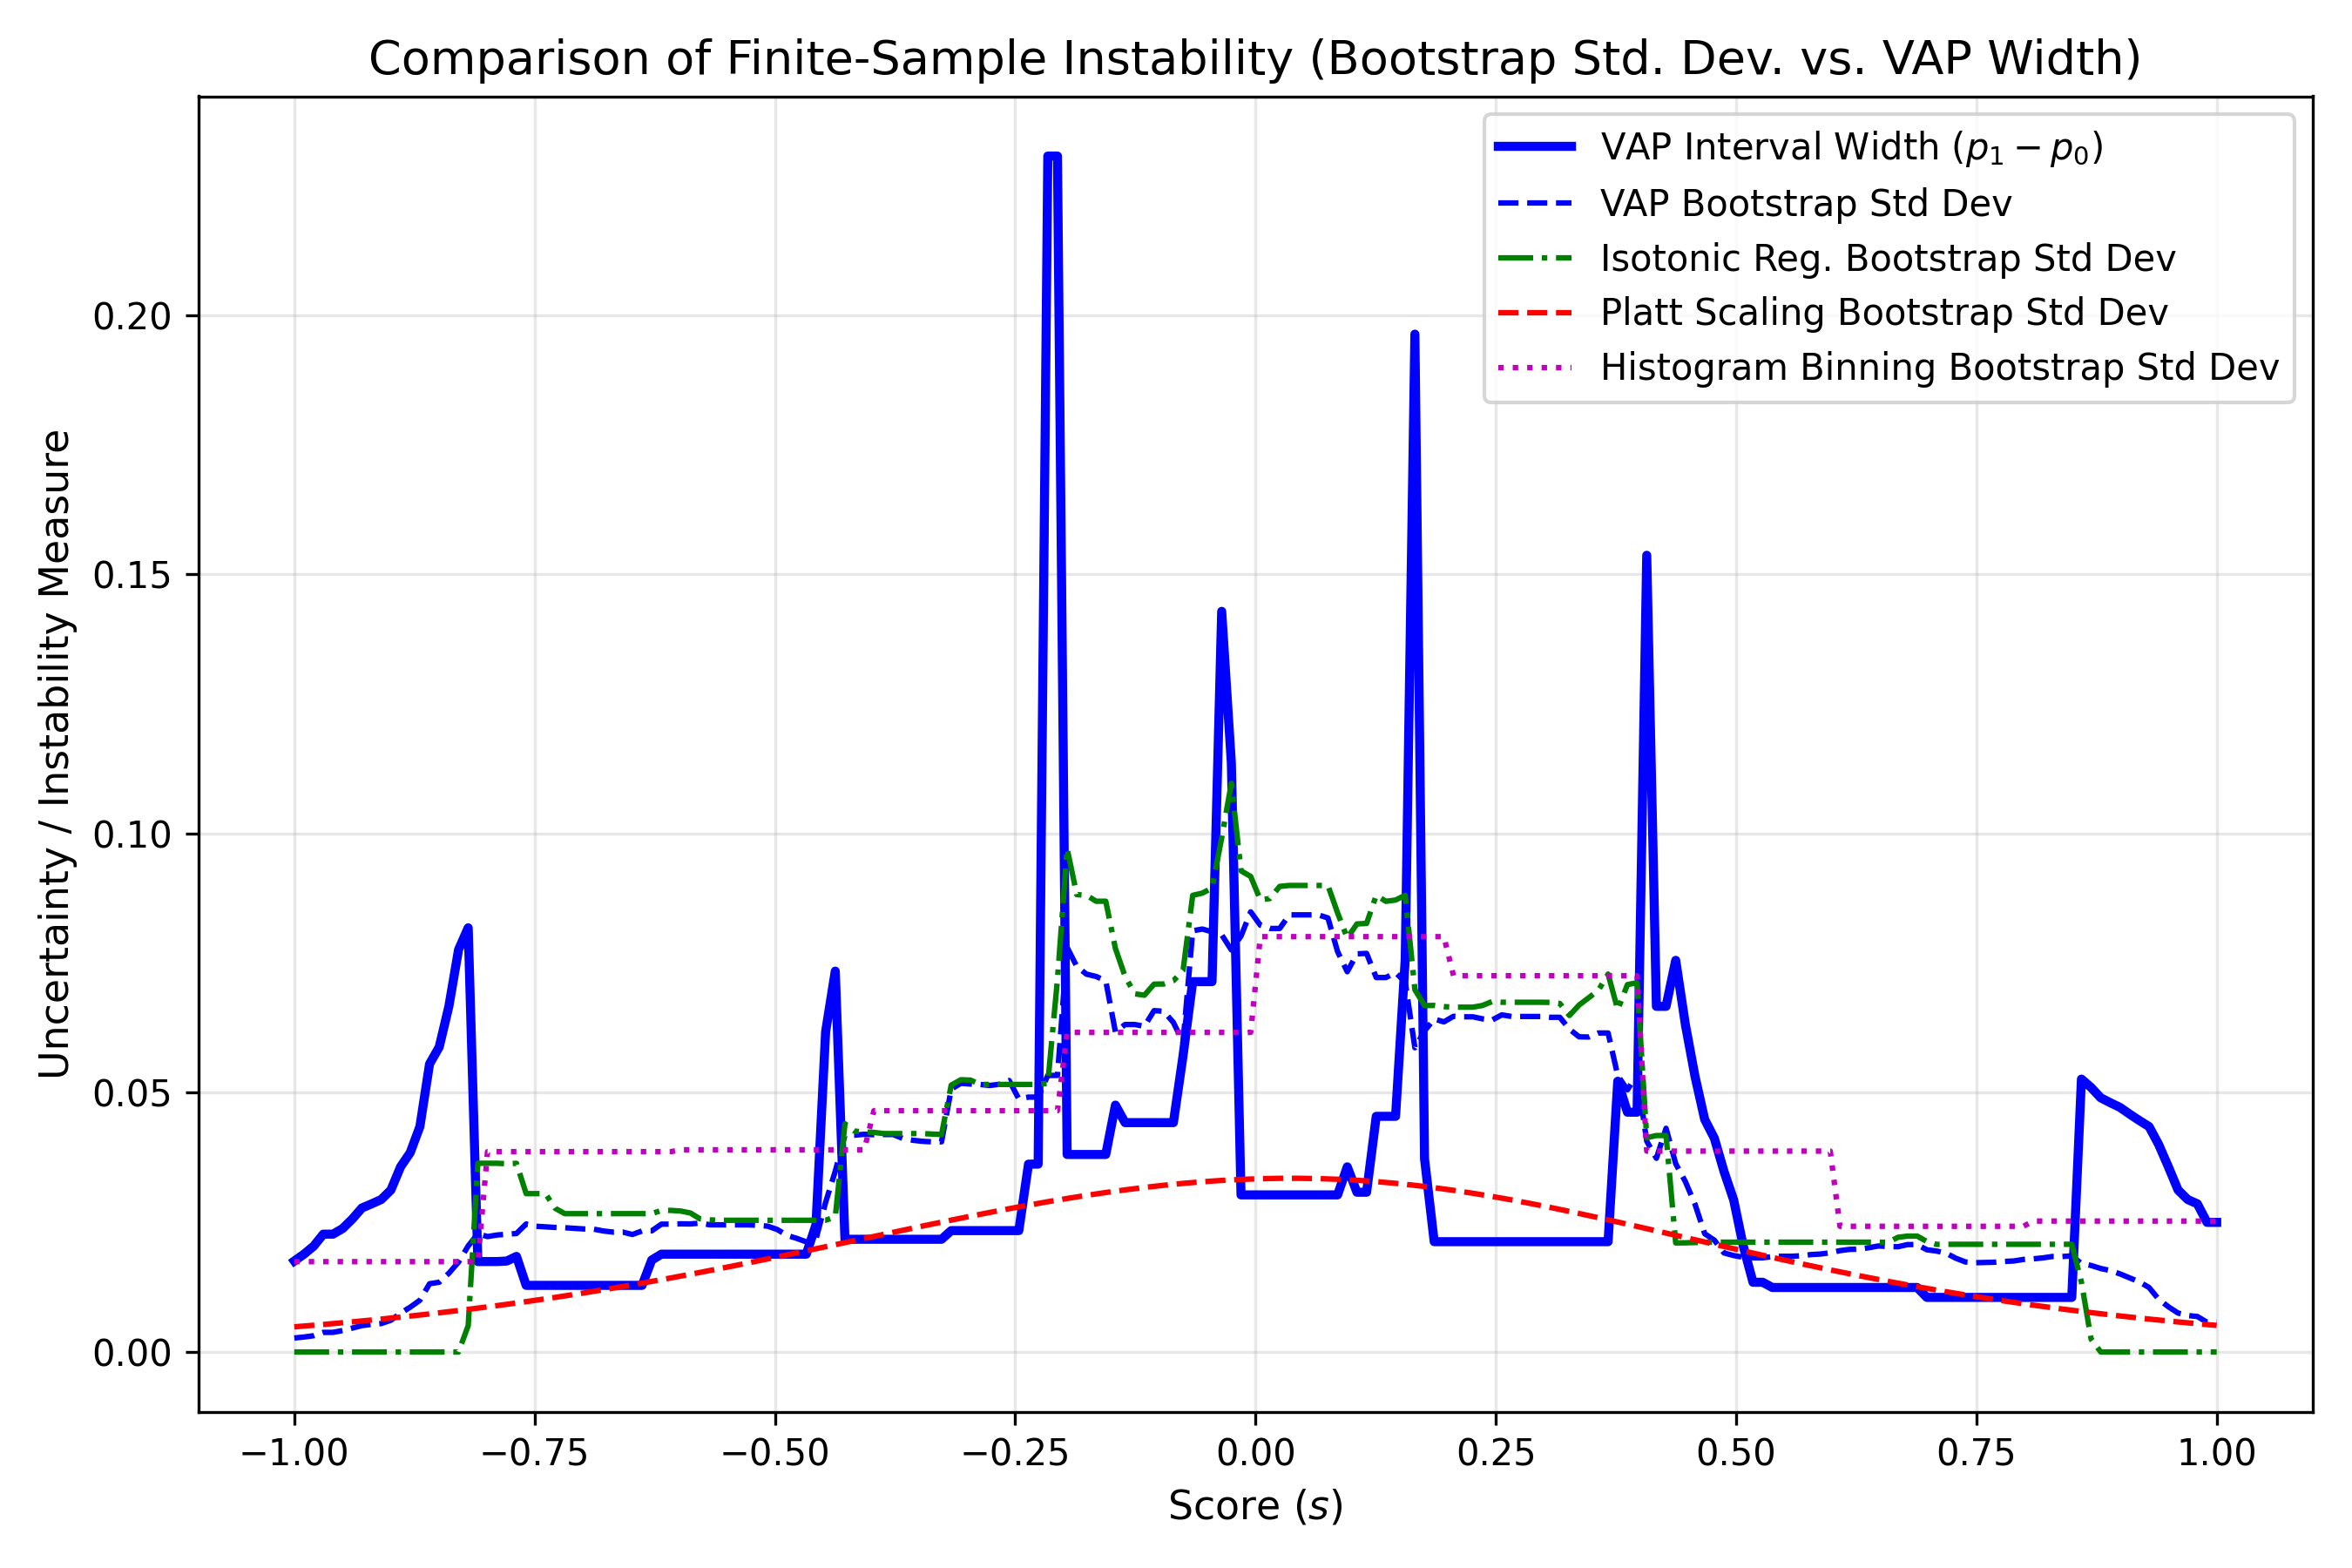
\includegraphics[width=0.85\textwidth]{calibration_uncertainty_bootstrap.png}
		\caption{Calibration instability across the four calibration methods. For Venn--Abers we also show the interval width $p_1-p_0$.}
		\label{fig:calibration_uncertainty_bootstrap}
	\end{figure}

	The Venn--Abers width and the bootstrap curves have a similar local structure, including spikes around changes in the fitted isotonic blocks. These are regions where relatively small changes in the calibration sample can alter the PAV partition and hence the fitted probability. The comparison is not intended to show that Venn--Abers width is numerically the same as a bootstrap standard deviation. It does, however, show that the width provides a local diagnostic of the sensitivity of the calibration fit without having to rerun the calibrator many times.


	% ============================================================
\section{Discussion and Practical Implications}
	\label{sec:discussion}

	The experiments suggest a more specific and limited interpretation of the Venn--Abers interval width than is often assumed in applications.

	The first point is the connection with the local PAV block. In a stable block containing $N$ observations, changing the hypothetical label of the test point changes the fitted probability by roughly $1/N$. The scaling experiments show the corresponding dependence on calibration size, score density, Bernoulli variance, and local slope. We therefore use the terms local calibration leverage or local calibration support for this quantity. We do not interpret it as a general measure of predictive epistemic uncertainty.

	Outcome ambiguity is a separate quantity. The $v^{-1/3}$ term in Proposition~1 is conditional on density and local slope, and these variables can move together in a fitted model. In the crowd-annotation experiment, width exhibits virtually zero correlation with annotator disagreement or entropy. Furthermore, on real tabular benchmarks, outcome ambiguity and calibration support width combine to explain finite-sample calibration instability, with width providing additional explanatory power ($\Delta R^2 > 0$). Width on its own should therefore not be used as a general indicator of ambiguous labels.

	It is equally essential to separate calibration support from base-model epistemic uncertainty. In our controlled thinning experiments, thinning the local calibration set monotonically increased width and calibration instability, while base-model epistemic uncertainty remained unchanged by construction. Conversely, subsampling the training set had a much larger effect on base-model uncertainty than on width for Adult and Bank, although width can also change because retraining alters the calibration-score geometry, as seen more clearly on Spambase. Thus:
	\begin{equation*}
		\text{outcome ambiguity} \neq \text{base-model epistemic uncertainty} \neq \text{calibration-support uncertainty}.
	\end{equation*}

	There is also a difference between width and the variability of the calibrated probability. The block argument gives an $n^{-2/3}$ rate for width but an $n^{-1/3}$ rate for the probability itself. The quantity
	\begin{equation}
		U_{\mathrm{cal}}=\sqrt{\hat p(1-\hat p)w}
	\end{equation}
	has the latter scale and performs better than raw width in the pointwise bootstrap experiment. The ratio between bootstrap SD and $U_{\mathrm{cal}}$ is not constant across all of the local regimes, however, so we regard $U_{\mathrm{cal}}$ as an instability index rather than as a general standard-error formula.

	The $n^{-2/3}$ relationship also gives a rough indication of how calibration sample size affects width. If the local regime remains unchanged, reducing a characteristic width by one half requires an increase in calibration sample size of approximately $2^{3/2}\approx2.83$. This is only a local calculation because the score density and shape of the calibration curve can also change when the calibration population changes.

	Finally, the non-monotonic experiments show another limitation of interpreting width as a general uncertainty score. Persistent violations can create large pooled PAV blocks and an $O(n^{-1})$ width regime. Higher-order flat monotone regions have their own rates. In both cases a small width can coexist with approximation error because the isotonic projection has pooled away local structure.

	\subsection{Limitations}
	The scaling relationships in this paper are heuristic rather than formal limit theorems. The large-$n$ experiment shows the finite-sample coefficients moving towards the proposed values, but this is empirical evidence and not a proof of convergence. $U_{\mathrm{cal}}$ has the predicted rate but is not an exact pointwise standard-error estimate. The crowd-annotation experiment is simulated rather than based on human annotator traces. A formal treatment of the pseudo-label path through changes in the PAV active blocks, together with extensions to multi-class Venn--Abers prediction, would be useful further work.

	% ============================================================
\section{Conclusion}
	\label{sec:conclusion}

	This paper investigated the meaning of the Venn--Abers interval width $w=p_1-p_0$. The main result is that the width can be understood through the local PAV block fitted by isotonic regression. In the regular monotonic case this gives
	\begin{equation}
		w_n(s)
		\propto
		n^{-2/3}f(s)^{-2/3}
		[\theta(s)(1-\theta(s))]^{-1/3}
		[\theta'(s)]^{2/3}.
	\end{equation}
	The simulation results recover the sample-size rate and show the finite-sample density, ambiguity, and slope coefficients getting closer to the proposed values as the calibration sample increases.

	The same argument also explains why interval width and probability-scale calibration instability are related but are not the same quantity. Width has the inverse-block $n^{-2/3}$ rate, while the fitted probability has the usual isotonic $n^{-1/3}$ rate. The corresponding index $U_{\mathrm{cal}}=\sqrt{\hat p(1-\hat p)w}$ follows the predicted rate and is more closely related to pointwise bootstrap instability than raw width in our experiments.

	The empirical results also show where this interpretation should stop. Width is not a direct measure of label ambiguity, distribution shift, or base-model parameter uncertainty. Across controlled experiments on real tabular benchmarks, reducing local calibration support increases Venn--Abers width and calibration instability while base-model uncertainty is held fixed by construction. The results suggest therefore that Venn--Abers width is most useful as an operational measure of local calibration leverage, increasing as effective local calibration support decreases, rather than as a general scalar uncertainty score.

	% ============================================================
	\appendix
	\section{Invariance of the Scaling Law Under Score Transformations}
	\label{sec:appendix_invariance}

	The heuristic scaling law of Equation~\ref{eq:scaling_law_final} is invariant under any strictly increasing transformation of the scores. We give two routes to this fact. First, invariance already holds for the underlying Venn--Abers procedure itself, exactly, for reasons that have nothing to do with the asymptotic block-size argument. Second, using this fact together with the score transformation $h=\theta$ shows that the general form of Equation~\ref{eq:scaling_law_final} is not an independent result requiring its own invariance check, but a corollary of the same law stated once, in the scale where the calibration curve is the identity.

	\subsection{Exact Invariance of the Venn--Abers Output}

	Let $h:\mathbb{R}\to\mathbb{R}$ be any strictly increasing function (distinct from the base scoring function $g$ of Section~\ref{sec:setup}, which is held fixed throughout this appendix) and let $s_{\text{new}}=h(s)$. Because $h$ is strictly increasing it is injective and order-preserving: for any two scores, $s_i<s_j \iff h(s_i)<h(s_j)$, and $s_i=s_j \iff h(s_i)=h(s_j)$. The PAV fits underlying $p_0(s)$ and $p_1(s)$ (Section~\ref{sec:venn_abers}) are computed entirely from the sorted order of the calibration scores, the tie structure among them, and the rank at which the test score is inserted; the numerical values of the scores play no other role. Consequently $h$ leaves every sort order, tie group, and insertion rank unchanged, so
	\begin{equation}
		p_0(h(s)) = p_0(s), \qquad p_1(h(s)) = p_1(s),
		\label{eq:exact_invariance}
	\end{equation}
	for the transformed calibration and test scores. This is an exact statement about the finite-sample Venn--Abers predictor, not merely about its asymptotic scaling law: the interval $[p_0,p_1]$ itself, not just Equation~\ref{eq:scaling_law_final}, is unchanged by any strictly increasing reparametrization of the scores.

	\subsection{The Scaling Law in Canonical Form}

	Equation~\ref{eq:exact_invariance} means the scaling law can be derived once, in a convenient reparametrization, with the general form recovered as a corollary. Suppose $\theta$ is strictly increasing on a neighbourhood of $s$, as already required for $\theta'(s)>0$ in Proposition~1, and let $h=\theta$ on that neighbourhood, defining canonical scores $P=\theta(S)$. Because $Y\mid S=s\sim\text{Bernoulli}(\theta(s))$ and $P=\theta(S)$ is a bijection there, $Y\mid P=p\sim\text{Bernoulli}(p)$ exactly: in canonical scale the calibration curve is the identity, $\theta_{\text{new}}(p)=p$ and $\theta_{\text{new}}'(p)=1$. By the usual change-of-variables rule, the canonical score density is
	\begin{equation}
		\varphi(\theta(s)) = \frac{f(s)}{\theta'(s)}.
		\label{eq:canonical_density}
	\end{equation}
	Substituting $\theta_{\text{new}}'=1$ into Equation~\ref{eq:scaling_law_final} removes the slope factor entirely, giving the simplified law
	\begin{equation}
		w_n(p) \propto n^{-2/3}\varphi(p)^{-2/3}[p(1-p)]^{-1/3},
		\label{eq:simplified_law}
	\end{equation}
	stated directly in the scale where the calibration curve is the identity, so no invariance question arises for it. Equation~\ref{eq:exact_invariance} guarantees $w_n(s)=w_n(\theta(s))$, so substituting Equation~\ref{eq:canonical_density} and $p=\theta(s)$ back into Equation~\ref{eq:simplified_law} recovers
	\begin{equation}
		w_n(s) \propto n^{-2/3}\left(\frac{f(s)}{\theta'(s)}\right)^{-2/3}[\theta(s)(1-\theta(s))]^{-1/3} = n^{-2/3}f(s)^{-2/3}[\theta(s)(1-\theta(s))]^{-1/3}[\theta'(s)]^{2/3},
		\label{eq:general_law_corollary}
	\end{equation}
	which is exactly Equation~\ref{eq:scaling_law_final}. The general scaling law is thus a corollary of Equation~\ref{eq:simplified_law} under $h=\theta$, rather than a separate result whose invariance under score transformations must be checked afterwards. Equation~\ref{eq:canonical_density} only requires $\theta'(s)\ne0$ locally near $s$; where $\theta$ is not globally monotone, $h$ need only agree with $\theta$ in a neighbourhood of $s$, since Proposition~1 is itself a purely local statement.

	\subsection{Flat Points and the General-Order Regime}

	The same canonical construction extends to the flat-point regime of Section~\ref{subsec:non_monotonic_theory}. If $\theta(s_0+u)-\theta(s_0)\asymp c\,\operatorname{sign}(u)|u|^{\alpha}$ for $\alpha>1$, then $h=\theta$ is still strictly increasing through $s_0$, so Equation~\ref{eq:exact_invariance} still applies, but $\theta'(s_0)=0$ and the canonical density is now singular at $p_0=\theta(s_0)$:
	\begin{equation}
		\varphi(q) \asymp f(s_0)\,c^{-1/\alpha}\,|q-p_0|^{1/\alpha-1}.
		\label{eq:singular_density}
	\end{equation}
	In canonical scale the calibration curve is still exactly the identity, so the local balance has no systematic-slope term to cancel; it is driven entirely by the singular local mass $N(\Delta)=n\int_{p_0-\Delta}^{p_0+\Delta}\varphi(q)\,dq \asymp nf(s_0)c^{-1/\alpha}\Delta^{1/\alpha}$. Balancing $\Delta$ against $\sqrt{v(p_0)/N(\Delta)}$, and mapping back through Equation~\ref{eq:exact_invariance} and $v(p_0)=v(s_0)$, gives
	\begin{equation}
		w_n(s_0) \propto [nf(s_0)]^{-\frac{2\alpha}{2\alpha+1}}v(s_0)^{-\frac{1}{2\alpha+1}}c^{\frac{2}{2\alpha+1}},
	\end{equation}
	which is exactly Equation~\ref{eq:general_order_scaling}. Equations~\ref{eq:scaling_law_final} and~\ref{eq:general_order_scaling} are therefore not two derivations connected only by a shared heuristic style: they are the same canonical bias--noise balance at $\alpha=1$ and at general $\alpha$, respectively. Both remain heuristic in the same sense as Proposition~1 -- the canonical reparametrization removes the invariance question, not the informality of the local bias--noise balance itself. The genuine monotonicity-violation regime of Equation~\ref{eq:scaling_law_violation} is unaffected by this construction: there $\theta$ is non-monotone on $I$, so no strictly increasing $h$ agreeing with $\theta$ on $I$ exists, and the population-level pooling argument of that regime applies instead.

	% ============================================================
	\section*{Acknowledgements}

	I thank Prof.\ Vladimir Vovk for useful discussions in writing this paper.

	% ============================================================
	\bibliographystyle{plain}
	\bibliography{references}
	
\end{document}
